\PassOptionsToPackage{unicode=true}{hyperref} % options for packages loaded elsewhere
\PassOptionsToPackage{hyphens}{url}
%
\documentclass[
]{book}
\usepackage{lmodern}
\usepackage{amssymb,amsmath}
\usepackage{ifxetex,ifluatex}
\ifnum 0\ifxetex 1\fi\ifluatex 1\fi=0 % if pdftex
  \usepackage[T1]{fontenc}
  \usepackage[utf8]{inputenc}
  \usepackage{textcomp} % provides euro and other symbols
\else % if luatex or xelatex
  \usepackage{unicode-math}
  \defaultfontfeatures{Scale=MatchLowercase}
  \defaultfontfeatures[\rmfamily]{Ligatures=TeX,Scale=1}
\fi
% use upquote if available, for straight quotes in verbatim environments
\IfFileExists{upquote.sty}{\usepackage{upquote}}{}
\IfFileExists{microtype.sty}{% use microtype if available
  \usepackage[]{microtype}
  \UseMicrotypeSet[protrusion]{basicmath} % disable protrusion for tt fonts
}{}
\makeatletter
\@ifundefined{KOMAClassName}{% if non-KOMA class
  \IfFileExists{parskip.sty}{%
    \usepackage{parskip}
  }{% else
    \setlength{\parindent}{0pt}
    \setlength{\parskip}{6pt plus 2pt minus 1pt}}
}{% if KOMA class
  \KOMAoptions{parskip=half}}
\makeatother
\usepackage{xcolor}
\IfFileExists{xurl.sty}{\usepackage{xurl}}{} % add URL line breaks if available
\IfFileExists{bookmark.sty}{\usepackage{bookmark}}{\usepackage{hyperref}}
\hypersetup{
  pdftitle={Alaska Region mdEditor Interim User Guide},
  pdfauthor={Alaska Region Data Stewardship Team},
  pdfborder={0 0 0},
  breaklinks=true}
\urlstyle{same}  % don't use monospace font for urls
\usepackage{longtable,booktabs}
% Allow footnotes in longtable head/foot
\IfFileExists{footnotehyper.sty}{\usepackage{footnotehyper}}{\usepackage{footnote}}
\makesavenoteenv{longtable}
\usepackage{graphicx,grffile}
\makeatletter
\def\maxwidth{\ifdim\Gin@nat@width>\linewidth\linewidth\else\Gin@nat@width\fi}
\def\maxheight{\ifdim\Gin@nat@height>\textheight\textheight\else\Gin@nat@height\fi}
\makeatother
% Scale images if necessary, so that they will not overflow the page
% margins by default, and it is still possible to overwrite the defaults
% using explicit options in \includegraphics[width, height, ...]{}
\setkeys{Gin}{width=\maxwidth,height=\maxheight,keepaspectratio}
\setlength{\emergencystretch}{3em}  % prevent overfull lines
\providecommand{\tightlist}{%
  \setlength{\itemsep}{0pt}\setlength{\parskip}{0pt}}
\setcounter{secnumdepth}{5}
% Redefines (sub)paragraphs to behave more like sections
\ifx\paragraph\undefined\else
  \let\oldparagraph\paragraph
  \renewcommand{\paragraph}[1]{\oldparagraph{#1}\mbox{}}
\fi
\ifx\subparagraph\undefined\else
  \let\oldsubparagraph\subparagraph
  \renewcommand{\subparagraph}[1]{\oldsubparagraph{#1}\mbox{}}
\fi

% set default figure placement to htbp
\makeatletter
\def\fps@figure{htbp}
\makeatother

\usepackage{booktabs}
\usepackage{longtable}
\usepackage[bf,singlelinecheck=off]{caption}

\usepackage{framed,color}
\definecolor{shadecolor}{RGB}{248,248,248}

\renewcommand{\textfraction}{0.05}
\renewcommand{\topfraction}{0.8}
\renewcommand{\bottomfraction}{0.8}
\renewcommand{\floatpagefraction}{0.75}

\renewenvironment{quote}{\begin{VF}}{\end{VF}}
\let\oldhref\href
\renewcommand{\href}[2]{#2\footnote{\url{#1}}}

\ifxetex
  \usepackage{letltxmacro}
  \setlength{\XeTeXLinkMargin}{1pt}
  \LetLtxMacro\SavedIncludeGraphics\includegraphics
  \def\includegraphics#1#{% #1 catches optional stuff (star/opt. arg.)
    \IncludeGraphicsAux{#1}%
  }%
  \newcommand*{\IncludeGraphicsAux}[2]{%
    \XeTeXLinkBox{%
      \SavedIncludeGraphics#1{#2}%
    }%
  }%
\fi

\makeatletter
\newenvironment{kframe}{%
\medskip{}
\setlength{\fboxsep}{.8em}
 \def\at@end@of@kframe{}%
 \ifinner\ifhmode%
  \def\at@end@of@kframe{\end{minipage}}%
  \begin{minipage}{\columnwidth}%
 \fi\fi%
 \def\FrameCommand##1{\hskip\@totalleftmargin \hskip-\fboxsep
 \colorbox{shadecolor}{##1}\hskip-\fboxsep
     % There is no \\@totalrightmargin, so:
     \hskip-\linewidth \hskip-\@totalleftmargin \hskip\columnwidth}%
 \MakeFramed {\advance\hsize-\width
   \@totalleftmargin\z@ \linewidth\hsize
   \@setminipage}}%
 {\par\unskip\endMakeFramed%
 \at@end@of@kframe}
\makeatother

\makeatletter
\@ifundefined{Shaded}{
}{\renewenvironment{Shaded}{\begin{kframe}}{\end{kframe}}}
\makeatother

\newenvironment{rmdblock}[1]
  {
  \begin{itemize}
  \renewcommand{\labelitemi}{
    \raisebox{-.7\height}[0pt][0pt]{
      {\setkeys{Gin}{width=3em,keepaspectratio}\includegraphics{images/#1}}
    }
  }
  \setlength{\fboxsep}{1em}
  \begin{kframe}
  \item
  }
  {
  \end{kframe}
  \end{itemize}
  }
\newenvironment{rmdnote}
  {\begin{rmdblock}{note}}
  {\end{rmdblock}}
\newenvironment{rmdcaution}
  {\begin{rmdblock}{caution}}
  {\end{rmdblock}}
\newenvironment{rmdimportant}
  {\begin{rmdblock}{important}}
  {\end{rmdblock}}
\newenvironment{rmdtip}
  {\begin{rmdblock}{tip}}
  {\end{rmdblock}}
\newenvironment{rmdwarning}
  {\begin{rmdblock}{warning}}
  {\end{rmdblock}}

\usepackage{makeidx}
\makeindex

\urlstyle{tt}

\usepackage{amsthm}
\makeatletter
\def\thm@space@setup{%
  \thm@preskip=8pt plus 2pt minus 4pt
  \thm@postskip=\thm@preskip
}
\makeatother

\frontmatter
\usepackage[]{natbib}
\bibliographystyle{apalike}

\title{Alaska Region mdEditor Interim User Guide}
\author{Alaska Region Data Stewardship Team}
\date{}

\begin{document}
\maketitle


%\cleardoublepage\newpage\thispagestyle{empty}\null
%\cleardoublepage\newpage\thispagestyle{empty}\null
%\cleardoublepage\newpage
\thispagestyle{empty}

\setlength{\abovedisplayskip}{-5pt}
\setlength{\abovedisplayshortskip}{-5pt}

{
\setcounter{tocdepth}{1}
\tableofcontents
}
\hypertarget{intro}{%
\chapter{Introduction}\label{intro}}

\begin{rmdcaution}
This is a working draft that will continue to be edited. Last updated:
2019-10-02. Please refresh this manual every time you open it to ensure
you are viewing the most recent version.
\end{rmdcaution}

The Alaska Region of the U.S. Fish and Wildlife Service is committed to improving the management of its data resources. A comprehensive, long-term plan to develop and implement a Regional Data Management System (RDMS) will begin in the winter of 2019, with the expectation that it will be fully operational and in use in 3-5 years. In the interim, there is a strong desire in the Region to begin managing existing and new data resources with the systems available to staff now.

This manual describes the INTERIM requirements and best practices for the creation of high-quality and consistent metadata records for projects and products from the Alaska Region (AK-Region) of the US Fish and Wildlife Service (USFWS). These metadata requirements conform to the standardized metadata format agreed upon by the Alaska Region Data Stewardship Team (DST). This metadata ensures that AK-Region projects and products are discoverable, accessible, and usable.

It is assumed that this manual will be continually revised and ultimately replaced following the development of the RDMS.

\hypertarget{metadata-and-mdeditor}{%
\section{Metadata and mdEditor}\label{metadata-and-mdeditor}}

The mdEditor is a metadata editing tool originally created to support the metadata requirements for USFWS Landscape Conservation Cooperatives as an extension of an initiative by the Alaska Data Integration Working Group (ADIwg). This tool was adopted by the AK-Region Regional Directorate Team, on the recommendation of the DST, to support the AK-Region's goal of improving data management.

This manual refers to the creation of AK-Region metadata specifically. If you want information on the creation of other metadata records using mdEditor, or more information in general, please refer to the mdEditor User Manual.

\hypertarget{who-should-use-this-manual}{%
\section{Who Should Use this Manual}\label{who-should-use-this-manual}}

This guide is for anyone creating or updating metadata for AK-Region projects and products. The primary purpose is to document items that are stored in project archive records, currently maintained on network drives and backed up with external hard drives.
The metadata requirements described here apply to science projects and products that were conducted or funded by the Fisheries and Ecological Services (FES), Migratory Bird Management (MBM), National Wildlife Refuge System (NWRS), or Office of Subsistence Management (OSM) branches of the Alaska Region.

\hypertarget{how-to-use-this-manual}{%
\section{How to Use this Manual}\label{how-to-use-this-manual}}

Directly accessing this manual from the internet is the recommended way to use this manual. By doing so, you will guarantee you are always using the current version since it is a live document and any updates can be made instantly. The online version will also have the best functionality and graphical display.

If needed, you can download this manual as a PDF and save a copy to your computer for printing or offline use. If you choose this method, be sure to reference the online version regularly and save a new PDF as updates are made to the online version. Also note that not all of the formatting will be exactly the same as the online version.

\hypertarget{disclaimer}{%
\section{Disclaimer}\label{disclaimer}}

This manual was developed while mdEditor is also undergoing development. Due to this, there may be minor discrepancies between screenshots in the manual and the current production version of mdEditor.

\mainmatter

\hypertarget{projects-products-and-contacts}{%
\chapter{Projects, Products, and Contacts}\label{projects-products-and-contacts}}

Contacts, projects, and products share a relationship in mdEditor and are each entered independently.

\hypertarget{projects}{%
\section{Projects}\label{projects}}

A project encompasses a discrete effort on a particular topic with defined goals or objectives. As an interim goal, target projects to undergo data management are science projects whose topics and resulting products have value to partners or the public being able to discover, access, and potentially use them.

\hypertarget{products}{%
\section{Products}\label{products}}

A product is a resource, usually (but not necessarily) developed as an output from a project. Products (aka Data Resources) are defined as recorded information and can be generated by experiments, models, simulations and observations. Not every output of a project is necessarily a product, however. For example, meeting minutes do not have standalone value as a publicly-available resource. Products that receive metadata records are at the discretion of the principal investigator, their supervisor and any relevant program or branch policies but should be guided by the principle of reuse (i.e., if there is an intent that a tabular dataset can be used again, it should be a product that undergoes data management; for reports, they should be managed to be discoverable and associated with the datasets and code used to produce results). Consider carefully why a product would remain in the project file but NOT undergo data management. This should be a rare occurrence.

\hypertarget{contacts}{%
\section{Contacts}\label{contacts}}

Contacts are the individuals and organizations involved with projects and products (e.g., collaborators, funders). Contacts are entered once in mdEditor and can be added to multiple projects and products.
Consult the contacts section for information on maintaining the contacts record and adding contacts.

\hypertarget{relationships}{%
\section{Relationships}\label{relationships}}

Projects and products will always have a relationship with contacts. Contacts can be individuals or organization. Projects will always have at least one point of contact. Additional contact relationships may include project authors, metadata creators, funders, principal investigators, publishers, distributors, and many others.
Contact types are specified in the contact record (examples: federal, state, NGO). Specific roles for each contact are defined within the respective project and product records (examples: principal investigator, collaborator).
Products are often the results of projects. mdEditor defines the relationships between projects and products through the Associated tab.

\hypertarget{workflow}{%
\chapter{Workflow}\label{workflow}}

The following is a suggested workflow for using mdEditor to create and save metadata records for AK-Region projects and products. Workflow can begin from scratch or by working with existing metadata records.

\hypertarget{from-scratch}{%
\section{From Scratch}\label{from-scratch}}

Follow this workflow if you do not have existing project or product metadata.

\hypertarget{step-1-gather-information-needed-for-your-metadata-entries.}{%
\subsection{Step 1: Gather information needed for your metadata entries.}\label{step-1-gather-information-needed-for-your-metadata-entries.}}

Have information about your contacts, projects, and products on hand before you begin creating metadata records. Key information to gather includes project proposals, project reports, product information, and contact information for individuals and organizations involved in the projects.

\hypertarget{step-2-open-mdeditor.}{%
\subsection{Step 2: Open mdEditor.}\label{step-2-open-mdeditor.}}

The direct link to mdEditor is \url{https://go.mdeditor.org}. Choose the browser you plan to use for mdEditor and bookmark this link.

mdEditor can also be accessed from its homepage at \url{https://www.mdeditor.org/}. This site provides some background information and Frequently Asked Questions about mdEditor.

\hypertarget{step-3-set-the-correct-default-settings.}{%
\subsection{\texorpdfstring{Step 3: Set the correct default \protect\hyperlink{settings}{Settings}.}{Step 3: Set the correct default Settings.}}\label{step-3-set-the-correct-default-settings.}}

{[} Under development {]}

\hypertarget{step-4-upload-or-create-contacts.}{%
\subsection{\texorpdfstring{Step 4: Upload or Create \protect\hyperlink{contact-entry-guidance}{Contacts}.}{Step 4: Upload or Create Contacts.}}\label{step-4-upload-or-create-contacts.}}

Contacts must be uploaded from the program archive folder or created before they can be added to project and product metadata records. See Contact Entry Guidance for more information.

\hypertarget{step-5-upload-data-dictionaries.}{%
\subsection{\texorpdfstring{Step 5: Upload \protect\hyperlink{dictionary-entry-guidance}{Data Dictionaries}.}{Step 5: Upload Data Dictionaries.}}\label{step-5-upload-data-dictionaries.}}

Upload existing data dictionaries from the program archive folder. If applicable, these can be reused across product metadata records.

\hypertarget{step-6-create-projects.}{%
\subsection{\texorpdfstring{Step 6: Create \protect\hyperlink{project-entry-guidance}{Projects}.}{Step 6: Create Projects.}}\label{step-6-create-projects.}}

Create an mdEditor project record from scratch.

\hypertarget{step-7-create-products.}{%
\subsection{\texorpdfstring{Step 7: Create \protect\hyperlink{product-entry-guidance}{Products}.}{Step 7: Create Products.}}\label{step-7-create-products.}}

Create an mdEditor product record from scratch.

\hypertarget{step-8-for-applicable-products-create-data-dictionaries.}{%
\subsection{\texorpdfstring{Step 8: For applicable Products, create \protect\hyperlink{dictionary-entry-guidance}{Data Dictionaries}.}{Step 8: For applicable Products, create Data Dictionaries.}}\label{step-8-for-applicable-products-create-data-dictionaries.}}

For tabular data products, if an existing data dictionary does not describe the product, create a new data dictionary.

\hypertarget{step-9-complete-metadata.}{%
\subsection{Step 9: Complete metadata.}\label{step-9-complete-metadata.}}

\hypertarget{step-10-create-desired-associations-between-projects-andor-products.}{%
\subsection{Step 10: Create desired Associations between Projects and/or Products.}\label{step-10-create-desired-associations-between-projects-andor-products.}}

Associations can be either associated from a project or associated from a product.

\hypertarget{step-11-publish-your-records-to-sciencebase.}{%
\subsection{Step 11: Publish your records to ScienceBase.}\label{step-11-publish-your-records-to-sciencebase.}}

{[} Under development {]}

\hypertarget{step-12-export-your-records-and-contacts-for-backup-transfer-or-sharing.}{%
\subsection{\texorpdfstring{Step 12: \protect\hyperlink{export}{Export} your records and contacts for backup, transfer, or sharing.}{Step 12: Export your records and contacts for backup, transfer, or sharing.}}\label{step-12-export-your-records-and-contacts-for-backup-transfer-or-sharing.}}

Export the project and product records to the project's archive folder (incoming folder) on your program's network drive. These records should be moved from your incoming folder to the metadata folder of the project by the data custodian. Rename this file ``project\_name.json.'' For example, MBMWF\_011\_YKDNestPlot.json would be the metadata record for the YK Delta nest plot survey project conducted by the Waterfowl Program in MBM (it was the 11th project archive record created by the program).

Separately export all contacts and all data dictionaries to the program's archive folder (root folder that contains all project archive folders).

\hypertarget{editing-and-re-export}{%
\section{Editing and Re-Export}\label{editing-and-re-export}}

Follow this workflow if you have already created metadata and need to update it.

\hypertarget{step-1-gather-information-needed-for-your-metadata-entries.-1}{%
\subsection{Step 1: Gather information needed for your metadata entries.}\label{step-1-gather-information-needed-for-your-metadata-entries.-1}}

Have the necessary information to update your metadata records readily accessible before you begin.

\hypertarget{step-2-open-mdeditor.-1}{%
\subsection{Step 2: Open mdEditor.}\label{step-2-open-mdeditor.-1}}

The direct link to mdEditor is \url{https://go.mdeditor.org}. Choose the browser you plan to use for mdEditor and bookmark this link.

mdEditor can also be accessed from its homepage at \url{https://www.mdeditor.org/}. This site provides some background information and Frequently Asked Questions about mdEditor.

\hypertarget{step-3-import-mdeditor-file.}{%
\subsection{\texorpdfstring{Step 3: \protect\hyperlink{import}{Import} mdEditor file.}{Step 3: Import mdEditor file.}}\label{step-3-import-mdeditor-file.}}

Import the mdEditor JSON file that you wish to edit from the project's archive folder.

\hypertarget{step-4-check-the-settings.}{%
\subsection{\texorpdfstring{Step 4: Check the \protect\hyperlink{settings}{Settings}.}{Step 4: Check the Settings.}}\label{step-4-check-the-settings.}}

{[} Under development {]}

\hypertarget{step-5-update-contacts.}{%
\subsection{\texorpdfstring{Step 5: Update \protect\hyperlink{contact-entry-guidance}{Contacts}.}{Step 5: Update Contacts.}}\label{step-5-update-contacts.}}

Import the Contact file from the program's archive folder. If you have new contacts to add to your metadata record, create those contacts and add them to the record.

\hypertarget{step-6-update-projects.}{%
\subsection{\texorpdfstring{Step 6: Update \protect\hyperlink{project-entry-guidance}{Projects}.}{Step 6: Update Projects.}}\label{step-6-update-projects.}}

Update/edit metadata as needed.

\hypertarget{step-7-update-products.}{%
\subsection{\texorpdfstring{Step 7: Update \protect\hyperlink{product-entry-guidance}{Products}.}{Step 7: Update Products.}}\label{step-7-update-products.}}

Update/edit metadata as needed.

\hypertarget{step-8-for-applicable-products-create-import-or-update-data-dictionaries.}{%
\subsection{\texorpdfstring{Step 8: For applicable Products, create, import, or update \protect\hyperlink{dictionary-entry-guidance}{Data Dictionaries}.}{Step 8: For applicable Products, create, import, or update Data Dictionaries.}}\label{step-8-for-applicable-products-create-import-or-update-data-dictionaries.}}

Import the Data Dictionaries file from the program's archive folder. If you have new data dictionaries to add to your metadata record, create those dictionaries and add them to the record.

\hypertarget{step-9-check-associations-between-projects-andor-products.}{%
\subsection{Step 9: Check Associations between Projects and/or Products.}\label{step-9-check-associations-between-projects-andor-products.}}

If you only updated metadata in existing records that were already associated, you do not need to do anything with the associations.

If you created a new product for your project, then associate those records in mdEditor.

\hypertarget{step-10-publish-your-records-to-sciencebase.}{%
\subsection{Step 10: Publish your records to ScienceBase.}\label{step-10-publish-your-records-to-sciencebase.}}

{[} Under development {]}

\hypertarget{step-11-export-your-records-and-contacts-for-backup-transfer-or-sharing.}{%
\subsection{\texorpdfstring{Step 11: \protect\hyperlink{export}{Export} your records and contacts for backup, transfer, or sharing.}{Step 11: Export your records and contacts for backup, transfer, or sharing.}}\label{step-11-export-your-records-and-contacts-for-backup-transfer-or-sharing.}}

Export the project and product records to the project's archive folder (incoming folder) on your program's network drive. These records should be moved from your incoming folder to the metadata folder of the project by the data custodian. Rename this file ``project\_name.json.'' For example, MBMWF\_011\_YKDNestPlot.json would be the metadata record for the YK Delta nest plot survey project conducted by the Waterfowl Program in MBM (it was the 11th project archive record created by the program).

Separately export all contacts and all data dictionaries back to the program's archive folder (root folder that contains all project archive folders).

\hypertarget{file-management}{%
\chapter{File Management}\label{file-management}}

File management in mdEditor consists of consistent and proper handling and storage of mdEditor derived formats of metadata. These files are essential for long-term access to metadata beyond a single work session.

\hypertarget{how-mdeditor-stores-information}{%
\section{How mdEditor Stores Information}\label{how-mdeditor-stores-information}}

mdEditor stores information on your local computer in your browser's localStorage cache (not the normal file cache). This means that if you use a different browser to access mdEditor, it will not show the metadata records from your original browser. It also means that clearing your browser's cache generally will not delete your mdEditor records. However, depending on your browser's settings, clearing your browser cache may still delete your mdEditor data (e.g., in Chrome, checking the ``\emph{cookies and other site data}'' option will clear your mdEditor data).

\begin{rmdcaution}
In mdEditor settings, you can clear your storage cache. Doing so will
remove all of the information currently loaded in mdEditor. Reasons you
might want to clear your storage cache is due to too much information
stored in the cache, or as a way to debug a problem with mdEditor.
\textbf{It is very important that you back up your records before
clearing the mdEditor cache to avoid losing your data}. Consult the
Export or Settings section of this manual to learn more.
\end{rmdcaution}

\hypertarget{mdeditor-file-format}{%
\section{mdEditor File Format}\label{mdeditor-file-format}}

JSON (JavaScript Object Notation) is an open-standard file format with file extension .json. The underlying format of the metadata from mdEditor is mdJSON, which was created specifically for mdEditor. There are two types of mdJSON files.

\begin{enumerate}
\def\labelenumi{\arabic{enumi}.}
\tightlist
\item
  \textbf{mdJSON} files are the format that is published from mdEditor and can be made available on ScienceBase and data.gov. Their default file name is \textbf{md\_metadata.json}.
\item
  \textbf{mdEditor} files are the files used by mdEditor and that are stored into the project's archive record. They contain extra information, such as settings, that tell mdEditor how to operate. Their default file name is \textbf{mdeditor-timestamp.json}.
\end{enumerate}

\begin{rmdtip}
mdEditor files will be exported and imported to/from the project's
archive record
\end{rmdtip}

\begin{center}\rule{0.5\linewidth}{\linethickness}\end{center}

\hypertarget{import}{%
\section{Import}\label{import}}

The Import function loads an mdEditor or mdJSON file into the current mdEditor session. You can also import existing ScienceBase metadata or FGDC (Federal Geographic Data Committee) metadata into mdEditor to create mdJSON.

\hypertarget{general-import-settings}{%
\subsection{General Import Settings}\label{general-import-settings}}

\hypertarget{replace-vs.-merge}{%
\subsubsection{Replace vs.~Merge}\label{replace-vs.-merge}}

The \textbf{Replace/Merge} toggle allows you to either replace or merge the imported records with the records currently loaded in mdEditor.

\begin{rmdtip}
When importing existing mdEditor files from the project archive folder,
choose ``Replace.'' That will ensure that only those records associated
with the project you are working on are loaded into the mdEditor.
\end{rmdtip}

\begin{rmdtip}
In most instances, when you import the Contacts or Data Dictionary
records, you should select ``Merge.'' That will ensure that the master
file of contacts or data dictionary records, stored in the program
archive folder, will be updated with any new entries added to the
mdEditor.
\end{rmdtip}

\hypertarget{import-screen}{%
\subsection{Import Screen}\label{import-screen}}

You can click or drag and drop a file onto the \textbf{Import Data} button to import a local file.

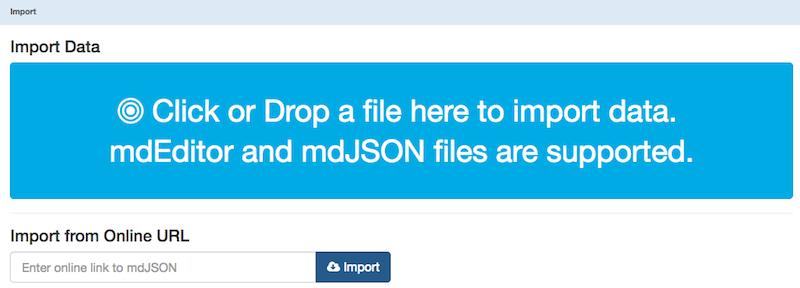
\includegraphics{images/import_window.png}

\begin{enumerate}
\def\labelenumi{\arabic{enumi}.}
\tightlist
\item
  Review the selected information. If there is more than one copy of the same metadata record or contact, use the ``preview JSON'' button to choose the record or contact with the most complete information.
\item
  Select the records you want to import.
\item
  Switch the Replace/Merge toggle to ``Replace'' for project/product records and ``Merge'' for Contact and Data Dictionary records.
\item
  Click on the right hand button ``Click to Import Data.''
\end{enumerate}

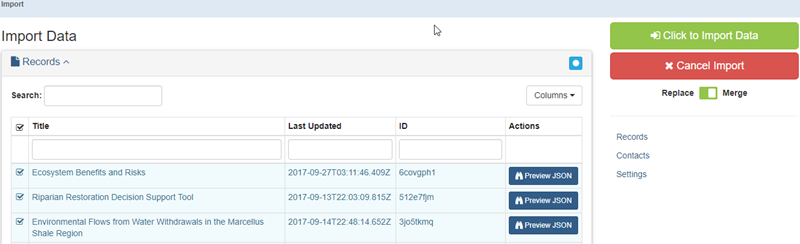
\includegraphics{images/import_data.png}

\begin{center}\rule{0.5\linewidth}{\linethickness}\end{center}

\hypertarget{export}{%
\section{Export}\label{export}}

The export function allows the current set of metadata records to be saved as an mdEditor or mdJSON file. The saved files can be shared with collaborators, imported into another record set, or imported into another browser. Exported mdEditor files should be saved as a backup or archival copy in the project's archive folder.

\hypertarget{using-export-to-backup-records}{%
\subsection{Using Export to Backup Records}\label{using-export-to-backup-records}}

Exporting records is the only way to save mdEditor files outside of your browser cache. You should backup by exporting an mdEditor JSON file each time you finish a work session in mdEditor or switch browsers.

\hypertarget{mdeditor-files-vs.-mdjson-files}{%
\subsubsection{mdEditor files vs.~mdJSON files}\label{mdeditor-files-vs.-mdjson-files}}

mdJSON files can be uploaded and translated to other formats via the mdTranslator application while mdEditor files are exclusive to the mdEditor application and retain all mdEditor information, including Settings.

\hypertarget{best-practices}{%
\subsubsection{Best Practices}\label{best-practices}}

-Export project and product records to the project's archive folder as an mdEditor JSON file. Include Settings.

-Export the contact and data dictionary records to the program's archive folder as mdEditor JSON files. Include Settings. These records are backed up in a different location because they are reused across many projects.

-It is particularly important that you export your records for backup before using mdEditor's Clear Storage Cache functionality (clearing the storage cache will delete any records or data you have entered into the mdEditor). Exporting ensures that your data is secure even after clearing the storage cache. Not exporting your data before clearing your cache will result in a permanent loss of records. Consult the Settings section of this manual to learn more.

\hypertarget{export-options}{%
\subsection{Export Options}\label{export-options}}

While exporting data, there are four options available (on the right side of the export data window).

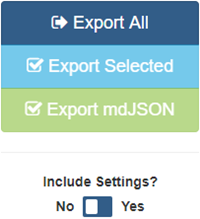
\includegraphics{images/export_data_action_menu.png}

\textbf{Export All}: will export everything currently loaded in mdEditor into a single file. Exports an mdEditor JSON file.

\textbf{Export Selected}: will only export the items you have selected (so individual records, contacts, etc.). If nothing is selected it will be disabled (i.e., grayed out). This exports an mdEditor JSON file.

\textbf{Export mdJSON}: only works for metadata records (i.e., doesn't work for contacts). Exports just the mdJSON file, which is a standalone JSON file you can load into mdTranslator and have translated into other metadata formats. mdJSON files imported into mdEditor are treated as new records and will not merge/update an existing record.

Clicking the \textbf{Include Settings} switch will also export mdEditor settings (only for mdEditor files). Consult the \protect\hyperlink{settings}{Settings} section of this manual to learn about settings.

\begin{center}\rule{0.5\linewidth}{\linethickness}\end{center}

\hypertarget{copy-records}{%
\section{Copy Records}\label{copy-records}}

The \textbf{Copy} button is located in the mdEditor action menu on the right-hand side of the screen. The Copy Button allows you to make a duplicate of an existing metadata record.

\textbf{Making a copy of a record can be used to:}

\begin{itemize}
\tightlist
\item
  Start a new product, project, or contact record.
\item
  Populate multiple products faster (e.g., multiple workshop reports, a poster based on a publication).
\item
  Create a ``template record'' for a project that can be used as a starting place for each full metadata record. A template record can contain information commonly used across your projects or products (such as contacts).
\end{itemize}

\textbf{Use the Copy button carefully}:

Making a copy will generate a new Record ID for the copied record and be named ``Copy of \ldots{}''. All the other info will remain the same \textbf{including associations}. The ``Metadata Identifier'' is NOT copied but any identifiers in the Main Citation \textbf{WILL be copied}.

\begin{rmdwarning}
It is extremely important to review all copied identifiers and delete
any that do not apply to the new record. Leaving in identifiers that do
not belong could result in your new item being published to the wrong
location.
\end{rmdwarning}

Before saving, carefully review all information in copied record to ensure all copied info is still relevant to the copied record, particularly any identifiers.

\hypertarget{settings}{%
\chapter{Settings}\label{settings}}

The settings menu allows for the configuring of user-specific options.

\hypertarget{general-settings}{%
\section{General Settings}\label{general-settings}}

\textbf{mdEditor Version}: The mdEditor version notes the current version of mdEditor. Use this when reporting errors. Errors can be reported at \url{https://github.com/adiwg/mdEditor/issues}. You must have a github account in order to post.

\textbf{Auto-Save}: The Auto-Save option will write all changes to local storage when you exit a data entry field. Changes must be manually saved if the Auto-Save feature is turned off.

Auto-Save allows you to save less frequently, but it makes it harder to undo changes that you make to your records. If you stay on the same record, you can cancel changes. But once you leave the record, the record is saved and you can't cancel the change except by manually re-editing the record.

\textbf{Clear All Records}: All records can be cleared by clicking the ``Clear Storage Cache.'' Be sure to back up all records (project and product records to the project's archive folder, contacts and data dictionaries to the program's archive folder) before clearing all records.

\begin{rmdcaution}
Clearing all records will delete all of the records currently loaded in
mdEditor. Before doing so, use the Export function to make a backup of
your records. Otherwise, the records will be permanently lost (unless
you previously made a backup copy).
\end{rmdcaution}

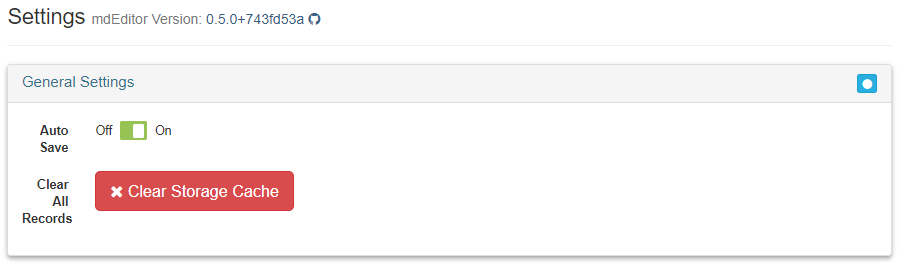
\includegraphics{images/settings-save-on.png}

\begin{center}\rule{0.5\linewidth}{\linethickness}\end{center}

\hypertarget{sciencebase-import-settings}{%
\section{ScienceBase Import Settings}\label{sciencebase-import-settings}}

{[}Under development{]}

\begin{center}\rule{0.5\linewidth}{\linethickness}\end{center}

\hypertarget{defaults}{%
\section{Defaults}\label{defaults}}

Defaults include settings for Language, Character Set, Country, and the \emph{Import URL }(used for defining the default URL for importing).

The following defaults will be pre-loaded:
- default language: English
- default character set: UTF-8
- default location: USA

Also included in \textbf{Defaults} are the \textbf{Metadata Repositories} (online databases for storing metadata). Once entered in \textbf{Settings} these can then be selected for projects and products so that they are flagged to a metadata repository of your choice.

\begin{center}\rule{0.5\linewidth}{\linethickness}\end{center}

\hypertarget{publishing-settings}{%
\section{Publishing Settings}\label{publishing-settings}}

{[}Under development{]}

\hypertarget{contact-entry-guidance}{%
\chapter{Contact Entry Guidance}\label{contact-entry-guidance}}

Contacts are individuals or organizations that can be referenced by projects or products. Contacts contain information such as the names of individuals or organizations, email address, physical address, website, and phone number so that viewers of metadata can communicate with those affiliated with a metadata record. Contacts also enable users to know who is involved in the creation and maintenance of projects and products, funding of projects, and creation and maintenance of metadata.

In mdEditor, contacts are created separately from individual records and are stored in the program's archive folder (root folder of all the project archive folders). Once contacts have been entered or imported into mdEditor, they can be used in any metadata record. See the File Management section for import and export guidance.

You should maintain a single list of your contacts. Having duplicate copies of the same contact is not desirable. It can create confusion as you edit and manage your metadata records and introduce unnecessary errors.

Copying contacts will change the ID and the name (the name will be ``Copy of \ldots{}.'') but all the other information will be the same.

\begin{rmdtip}
It is recommended that you export all Contacts to the program's archive
folder at the end of each working session and import them before a new
session begins (see File Management). This allows for the generation of
a single list of contacts for the program that multiple metadata authors
can use. Always spell out acronyms and organization names.
\end{rmdtip}

\begin{rmdcaution}
Make sure your contacts are loaded and accurate in mdEditor before
creating or editing your metadata records.
\end{rmdcaution}

\begin{center}\rule{0.5\linewidth}{\linethickness}\end{center}

\hypertarget{individual-contacts}{%
\section{Individual Contacts}\label{individual-contacts}}

\begin{enumerate}
\def\labelenumi{\arabic{enumi}.}
\tightlist
\item
  Click the
  
\includegraphics[width=0.22in]{images/symbol_plus_16} by Contacts.
\item
  Specify the contact is an Individual.
\item
  The Contact ID will be auto-generated by mdEditor.
\end{enumerate}

\emph{The following fields are available for Individual Contacts}:

\begin{itemize}
\item
  \textbf{Individual Name} (\emph{Required}): Enter individual's full name If you are entering a generic Individual contact, you can enter a Position Name without entering an Individual Name. For example: you could enter I\&M Data Manager as a Position Name rather than an Individual Name.
\item
  \textbf{Position Name} (\emph{Required}): Enter individual's full title; avoid acronyms If you have entered the individual's name, Position Name is not required (one or the other is required, but not both).
\item
  \textbf{Contact Type} (\emph{Required}): Enter the contact type from the picklist. Make sure every contact has Contact Type selected.
\item
  \textbf{Member Organization} (\emph{Required}): Select organization(s). You can make an individual part of multiple organizations.
\item
  \textbf{Email Address} (\emph{Required}): Enter individual's email
\item
  \textbf{Physical Address} (\emph{Best Practice}): Enter a physical address
\item
  \textbf{Logo} (\emph{Optional}):

  \begin{itemize}
  \tightlist
  \item
    It is uncommon that you would add a logo for an individual. If the individual is part of an organization, the individual will inherit the logo from the organization.
  \item
    You can either select or drop an image. If you choose to load an image, mdEditor will create a URI and will have a size limit for the logo. If you have a larger image, link to it rather than loading it into mdEditor.
  \end{itemize}
\end{itemize}

If you upload a logo to your contact record, you must include a filename for the logo. Otherwise you will get an error on the metadata records that include that contact.

\begin{center}\rule{0.5\linewidth}{\linethickness}\end{center}

\hypertarget{organization-contacts}{%
\section{Organization Contacts}\label{organization-contacts}}

\begin{enumerate}
\def\labelenumi{\arabic{enumi}.}
\tightlist
\item
  Click the
  
\includegraphics[width=0.22in]{images/symbol_plus_16} by \textbf{Contacts}.
\item
  Specify the contact is an \textbf{Organization}.
\item
  The \textbf{Contact ID} will be auto-generated by mdEditor.
\end{enumerate}

\emph{The following fields are available for} \textbf{Organization Contacts}:

\begin{itemize}
\item
  \textbf{Organization Name} (\emph{Required}): The organization's full name; avoid acronyms (however, abbreviating United States as U.S. is acceptable. Example: U.S. Fish and Wildlife Service).
\item
  \textbf{Contact Type} (\emph{Required}): Enter the contact type from the picklist. Make sure every contact has Contact Type selected.
\item
  \textbf{Email Address} (\emph{Required}): Add an email address of the primary contact in the organization.
\item
  \textbf{Online Resource} (\emph{Required}): Add a web URL where the organization resides. Online resource may also include social networks.
\item
  \textbf{Physical Address} (\emph{Best Practice}): Enter a physical address
\item
  \textbf{Logo} (\emph{Optional}):

  \begin{itemize}
  \tightlist
  \item
    You can either select or drop an image. If you choose to load an image, mdEditor will create a URI and will have a size limit for the logo. If you have a larger image, link to it rather than loading it into mdEditor.
  \item
    If an organization has a logo associated with it, individuals will inherit the logos from the organization.
  \end{itemize}
\end{itemize}

\begin{rmdwarning}
If you upload a logo to your contact record, you must include a filename
for the logo. Otherwise you will get an error on the metadata records
that include that contact.
\end{rmdwarning}

\hypertarget{dictionary-entry-guidance}{%
\chapter{Dictionary Entry Guidance}\label{dictionary-entry-guidance}}

Data dictionaries define the characteristics of attributes (also called variables or column names) that make up an entity (also called a table). A single data dictionary can describe the attributes of a single table or a collection of tables, like a database. Like Contacts, data dictionaries are created separately from Product records. Also like Contacts, dictionaries can be reused across products and are stored outside the project archive folder in the program archive folder.

It is recommended that you export all Data dictionaries to the program's archive folder at the end of each working session and import them before a new session begins (see \protect\hyperlink{file-management}{File Management}). This allows for the generation of a single list of dictionaries for the program that multiple metadata authors can use.

After a data dictionary has been described, it can be added to the product metadata record (see \protect\hyperlink{dictionaries-tab}{Dictionaries} tab).

\begin{center}\rule{0.5\linewidth}{\linethickness}\end{center}

\hypertarget{creating-a-new-data-dictionary}{%
\section{Creating a New Data Dictionary}\label{creating-a-new-data-dictionary}}

If an existing data dictionary does not describe the product you are working on, create a new data dictionary by clicking the

\includegraphics[width=0.22in]{images/symbol_plus_16} by \textbf{Dictionaries}.

Give the dictionary a title and chose \textbf{tabularDataset} as the subject.

\begin{rmdtip}
Meaningful titles will help link the data dictionary to its product(s)
while building the product metadata record.
\end{rmdtip}

Click \textbf{Save}.

\begin{center}\rule{0.5\linewidth}{\linethickness}\end{center}

\hypertarget{main-tab}{%
\section{Main Tab}\label{main-tab}}

\begin{longtable}[]{@{}ll@{}}
\toprule
Quick Reference: Dictionary Main Tab & Required?\tabularnewline
\midrule
\endhead
Basic Information: Title, Subject & Required\tabularnewline
Responsible Party & Required\tabularnewline
\bottomrule
\end{longtable}

\hypertarget{responsible-party-required}{%
\subsection{Responsible Party (Required)}\label{responsible-party-required}}

Adding a point of contact gives users information on who to contact should they have a question regarding your dictionary.

\begin{rmdtip}
To add contacts to a metadata record, you must first create/upload the
contacts into mdEditor. See the Contact Section for more information.
\end{rmdtip}

\begin{longtable}[]{@{}lll@{}}
\toprule
Role & Contact & Required?\tabularnewline
\midrule
\endhead
pointOfContact & Identified in Roles and Responsibilities & Required\tabularnewline
author & Identified in Roles and Responsibilities & Best Practice\tabularnewline
principalInvestigator & The Project PI & Best Practice\tabularnewline
\bottomrule
\end{longtable}

The point of contact for a project should be identified with Roles and Responsibilities (see Interim DM Implementation Guide). This is an interim solution as the point of contact can become obsolete if there is a positional change within an organization.

\begin{center}\rule{0.5\linewidth}{\linethickness}\end{center}

\hypertarget{citation-tab}{%
\section{Citation Tab}\label{citation-tab}}

\begin{longtable}[]{@{}ll@{}}
\toprule
Quick Reference: Dictionary Citation Tab & Required?\tabularnewline
\midrule
\endhead
Title & Required\tabularnewline
Date & Best Practice\tabularnewline
Responsible Parties & Required\tabularnewline
\bottomrule
\end{longtable}

\hypertarget{dates-best-practice}{%
\subsection{Dates (Best Practice)}\label{dates-best-practice}}

Add at least one date. Recommended are ``creation'' (when you first created your dictionary) and ``lastUpdate'' (when you updated the dictionary after initial publication).

\hypertarget{responsible-parties-required}{%
\subsection{Responsible Parties (Required)}\label{responsible-parties-required}}

\textbf{Responsible Parties} are required. Adding these will give users a contact point should they have any questions about the dictionary.

\begin{longtable}[]{@{}lll@{}}
\toprule
Role & Contact & Required?\tabularnewline
\midrule
\endhead
author & Identified in Roles and Responsibilities & At least one is required\tabularnewline
pointOfContact & Identified in Roles and Responsibilities & Required\tabularnewline
\bottomrule
\end{longtable}

\begin{center}\rule{0.5\linewidth}{\linethickness}\end{center}

\hypertarget{entities-tab}{%
\section{Entities Tab}\label{entities-tab}}

An Entity is a table. More than one entity can be described by a single data dictionary, as with a database.

Using the ``Import CSV'' button in the Entities Tab will allow you to pre-populate information in your data dictionary with the tabular dataset(s) you are documenting.

\begin{rmdtip}
Using the ``Import CSV'' functionality is highly recommended to start
defining a data dictionary.
\end{rmdtip}

Click ``Import CSV'' on the right hand side of the window. Either navigate to the tabular dataset you are documenting or drag-and-drop the file.

Check that the Names and Data Types were correctly imported. Check ``Domain'' box for an attribute if you wish to limit the entries allowed for the attribute (for example, allowing ``Female'' and ``Male'' for the attribute ``Sex''). Check ``Allow Null'' values if the attribute is allowed to have missing entries. Check ``Max/Min'' if you would like to set maximum and minimum values for the attribute.

After checking each attribute for these characteristics, click ``Do Import.''

Repeat this process for each entity that is described by the data dictionary.

\hypertarget{entity-information}{%
\subsection{Entity Information}\label{entity-information}}

Give a name to the entity in ``Code Name'' and a brief definition for the entity.

\hypertarget{attributes}{%
\subsection{Attributes}\label{attributes}}

The attributes (variables or column names) imported from the tabular dataset will be listed in a table and you must provide a brief definition for each. Additional information about the attribute can be described by clicking ``More.''

\begin{center}\rule{0.5\linewidth}{\linethickness}\end{center}

\hypertarget{domain-tab}{%
\section{Domain Tab}\label{domain-tab}}

Domains are discrete, allowable values that an attribute might take. For example, the attribute ``Color'' in a table may only be allowed to take values ``Red,'' ``Green,'' and ``Yellow.''

Each attribute that you checked the ``Domain'' box for during csv import (see the \protect\hyperlink{entities-tab}{Entities Tab} for import guidance) will be listed in a table under the Domain tab. For each, you must describe the allowable domains.

Click ``More'' for each attribute. Give the attribute a short description in the Domain Information box (this can be the same definition provided for it in the Entities tab).

Under Domain Items, give a short definition for each allowable domain.

Click ``Back to Domains'' and repeat for each attribute requiring defined domains.

\hypertarget{project-entry-guidance}{%
\chapter{Project Entry Guidance}\label{project-entry-guidance}}

The Project Entry Guidance section will cover how to create a metadata record for an AK-Region project.

\begin{center}\rule{0.5\linewidth}{\linethickness}\end{center}

\hypertarget{before-you-begin}{%
\section{Before You Begin}\label{before-you-begin}}

\hypertarget{select-the-lccproject-profile}{%
\subsection{Select the lccProject Profile:}\label{select-the-lccproject-profile}}

After creating your project record and before you begin adding metadata, select \textbf{lccProject} from the \textbf{Profile} drop-down in the main menu. This will limit the number of available tabs and only show tabs that contain fields that are applicable to project metadata.

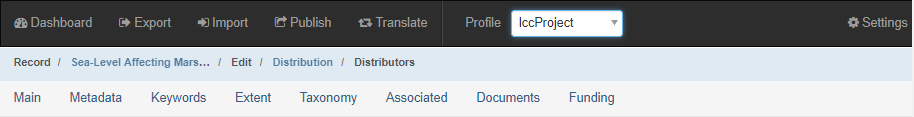
\includegraphics{images/profile_lccproject.png}

\hypertarget{make-sure-your-contacts-are-loaded-into-mdeditor}{%
\subsection{\texorpdfstring{Make sure your \protect\hyperlink{contact_entry_guidance}{contacts} are loaded into mdEditor:}{Make sure your contacts are loaded into mdEditor:}}\label{make-sure-your-contacts-are-loaded-into-mdeditor}}

In mdEditor, contacts are created separately from individual records and then stored within a library in mdEditor. Once contacts have been entered or imported into mdEditor, they can be used in any metadata records.

You should maintain a single list of your contacts in the program's archive folder (root folder that contains all project archive folders). Having duplicate copies of the same contact is not desirable. It can create confusion as you edit and manage your metadata records and introduce unnecessary errors.

\begin{center}\rule{0.5\linewidth}{\linethickness}\end{center}

\hypertarget{edit-a-project}{%
\section{Edit a Project}\label{edit-a-project}}

\begin{enumerate}
\def\labelenumi{\arabic{enumi}.}
\tightlist
\item
  Import or create your project record (see \protect\hyperlink{workflow}{workflow}).
\item
  Pick ``project'' as the Resource Type
\item
  Select the lccProject Profile: from the Main Menu (Top Navigation Bar) select ``lccProject'' from the profile drop-down menu.
\item
  Fill out metadata information for the following tabs:
\end{enumerate}

\begin{itemize}
\tightlist
\item
  \protect\hyperlink{project-main}{Main Tab}
\item
  \protect\hyperlink{project-metadata}{Metadata Tab}
\item
  \protect\hyperlink{project-keywords}{Keywords Tab}
\item
  \protect\hyperlink{project-extent}{Extent Tab}
\item
  \protect\hyperlink{project-taxonomy}{Taxonomy Tab}
\end{itemize}

\begin{enumerate}
\def\labelenumi{\arabic{enumi}.}
\setcounter{enumi}{4}
\tightlist
\item
  If applicable, \protect\hyperlink{project-associations}{associate} your project with other metadata records.
\end{enumerate}

\hypertarget{required-and-best-practice-fields-for-projects}{%
\section{Required and Best Practice Fields for Projects}\label{required-and-best-practice-fields-for-projects}}

\hypertarget{main-tab-1}{%
\subsection{Main Tab}\label{main-tab-1}}

\begin{itemize}
\tightlist
\item
  Basic Information: Title, Status, Language
\item
  Resource Type
\item
  Point of Contact
\item
  Main Citation

  \begin{itemize}
  \tightlist
  \item
    Identifier
  \item
    Responsible Parties
  \end{itemize}
\item
  Description

  \begin{itemize}
  \tightlist
  \item
    Abstract
  \end{itemize}
\item
  Time Period

  \begin{itemize}
  \tightlist
  \item
    Start Date
  \item
    End Date
  \end{itemize}
\end{itemize}

\hypertarget{metadata-tab}{%
\subsection{Metadata Tab}\label{metadata-tab}}

\begin{itemize}
\tightlist
\item
  Basic Information: Status, Dates
\item
  Metadata Contacts
\item
  Metadata Identifier
\end{itemize}

\hypertarget{keywords-tab}{%
\subsection{Keywords Tab}\label{keywords-tab}}

\begin{itemize}
\tightlist
\item
  ISO Topic Category
\item
  GCMD Keywords
\end{itemize}

\hypertarget{extent-tab}{%
\subsection{Extent Tab}\label{extent-tab}}

\begin{itemize}
\tightlist
\item
  Geographic Extent
\end{itemize}

\hypertarget{taxonomy-tab}{%
\subsection{Taxonomy Tab}\label{taxonomy-tab}}

\begin{itemize}
\tightlist
\item
  Taxonomic classifications
\end{itemize}

\begin{center}\rule{0.5\linewidth}{\linethickness}\end{center}

\hypertarget{project-main}{%
\section{Main Tab}\label{project-main}}

The Main tab allows for the creation and/or editing of primary metadata.

\begin{longtable}[]{@{}ll@{}}
\toprule
Quick Reference: Project Main Tab & Required?\tabularnewline
\midrule
\endhead
Basic Information: Title, Status & Required\tabularnewline
Resource Type & Required\tabularnewline
Point of Contact & Required\tabularnewline
Citation: Responsible Parties, Identifier & Required\tabularnewline
Time Period: Start Date, End Date & Required\tabularnewline
\bottomrule
\end{longtable}

\hypertarget{basic-information}{%
\subsection{Basic Information}\label{basic-information}}

\hypertarget{record-id}{%
\subsubsection{Record ID}\label{record-id}}

Record ID will be auto-generated. It can be edited but it should only be edited if absolutely necessary (and ideally edited as soon as the record is created in mdEditor).

\hypertarget{title-required}{%
\subsubsection{Title (Required)}\label{title-required}}

Enter as informative a title as possible. Good titles, when they appear in a search, will be understood and/or traceable.

\hypertarget{status-required}{%
\subsubsection{Status (Required)}\label{status-required}}

The Status drop-down menu allows you to select the status of your project. Choose status ONLY from the four following options: completed, ongoing, proposed, or accepted.

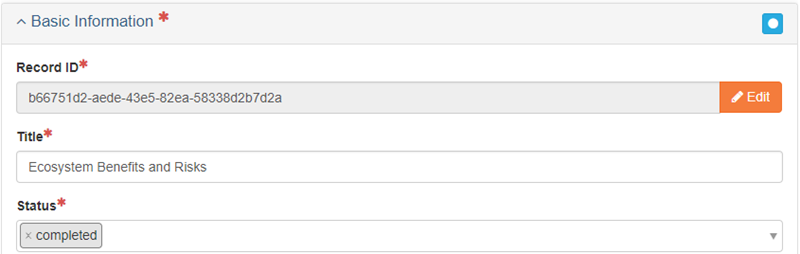
\includegraphics{images/main_screenshot_updated.png}

\hypertarget{default-locale}{%
\subsubsection{Default Locale}\label{default-locale}}

\textbf{Default Locale} allows for the selection of \textbf{Language, Character Set}, and \textbf{Country}. English, UTF-8, and USA will be selected by default, but you may change them if necessary.

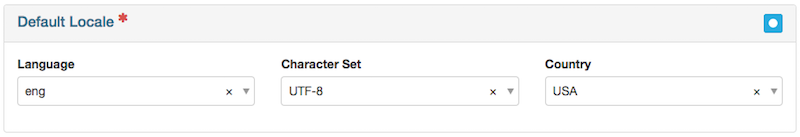
\includegraphics{images/default_locale.png}

\hypertarget{resource-types-required}{%
\subsubsection{Resource Types (Required)}\label{resource-types-required}}

For projects, the Resource Type should be automatically filled in with the resource type you selected when you created your record. This should be ``project'' for all AK-Region projects. Name is optional. You can leave this blank or use the Short Title from the archive record.

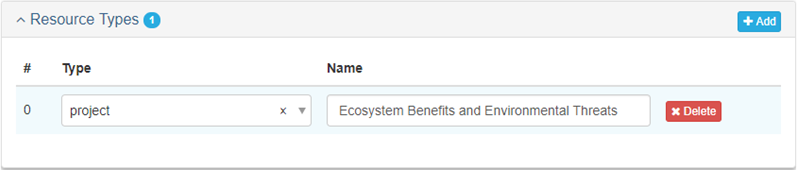
\includegraphics{images/resource_types.png}

\hypertarget{points-of-contact}{%
\subsubsection{Points of Contact}\label{points-of-contact}}

Adding a point of contact gives users information on who to contact should they have a question regarding your project or product.

\begin{rmdtip}
To add contacts to a metadata record, you must first create/upload the
contacts into mdEditor. See the Contact Section for more information.
\end{rmdtip}

\hypertarget{contacts-1}{%
\paragraph{Contacts}\label{contacts-1}}

\begin{longtable}[]{@{}lll@{}}
\toprule
Role & Contact & Required?\tabularnewline
\midrule
\endhead
pointOfContact & Identified in Roles and Responsibilities & Required\tabularnewline
principalInvestigator & The Project PI & Best Practice\tabularnewline
\bottomrule
\end{longtable}

The point of contact for a project should be identified with Roles and Responsibilities (see Interim DM Implementation Guide). This is an interim solution as the point of contact can become obsolete if there is a positional change within an organization.

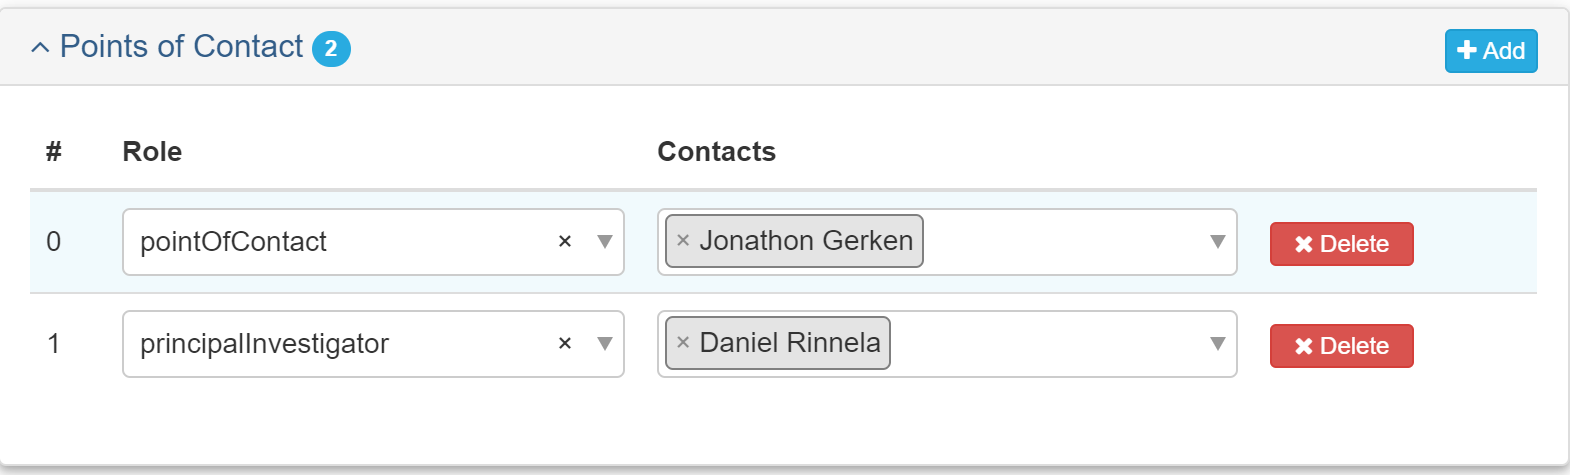
\includegraphics{images/contacts_image.png}

\hypertarget{citation}{%
\subsection{Citation}\label{citation}}

The \textbf{Citation} describes pertinent information about your project such as: responsible parties, internal identifiers, and any online resources that may relate to your item. Adding information in the citation will also improve users' ability to find your items.

\hypertarget{citation-required-fields}{%
\subsubsection{Citation Required Fields}\label{citation-required-fields}}

\textbf{Title (Required)}
The citation title is automatically populated with the title of your record.

\textbf{Alternate Title (Optional)}
You can add an alternate title if desired, such as the Short Title used in the archive record.

\textbf{Dates (Optional)}
Enter acquisition, creation, revision, or another date reference from the picklist and then enter the date.

\textbf{Responsible Parties (Required)}
Responsible parties must include a point of contact, but may also include the other responsible parties identified in Roles and Responsibilities (see Interim DM Implementation Guide) such as custodian, editor (data steward), and administrator.

\begin{rmdtip}
To add contacts to a metadata record, you must first create/upload the
contacts in mdEditor. See the Contacts section for more information.
\end{rmdtip}

\begin{longtable}[]{@{}lll@{}}
\toprule
Role & Contact & Required?\tabularnewline
\midrule
\endhead
pointOfContact & Identified in Roles and Responsibilities & Required\tabularnewline
custodian & Identified in Roles and Responsibilities & Best Practice\tabularnewline
editor & Identified in Roles and Responsibilities & Best Practice\tabularnewline
administrator & Identified in Roles and Responsibilities & Best Practice\tabularnewline
\bottomrule
\end{longtable}

\textbf{Online Resource (Required, if available)}
Enter the Name and URL for the project homepage, if available.

\textbf{Identifier (Best Practice)}
You may enter as many identifiers as desired. At a minimum, include the full archive record name here. Example: AFB\_001\_SockeyeFyke

\hypertarget{description}{%
\subsection{Description}\label{description}}

\textbf{Description} allows for the addition of the \textbf{Abstract} as well as a Short Abstract, and Supplemental Information.

\hypertarget{abstract-required}{%
\subsubsection{Abstract (Required)}\label{abstract-required}}

Enter an abstract that succinctly describes the project's purpose and goals. Include key species or habitats as well.

\begin{rmdtip}
Write your project abstract in the present tense if the project is in
progress and past tense if the project has been completed.
\end{rmdtip}

\hypertarget{short-abstract-optional}{%
\subsubsection{Short Abstract (Optional)}\label{short-abstract-optional}}

Enter a short description, limited to 300 characters, if desired.

Enter comments, if desired.

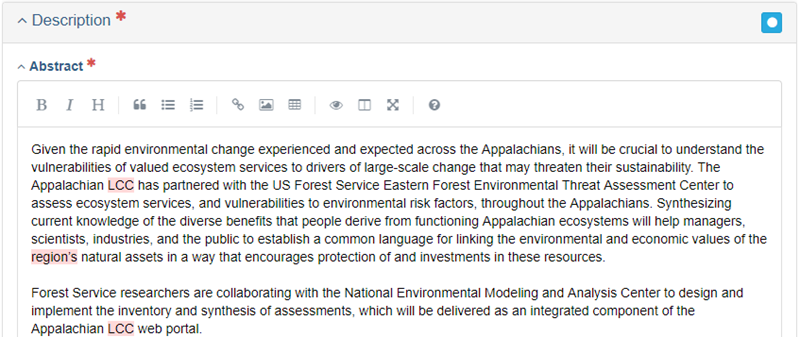
\includegraphics{images/description_lcc.png}

\hypertarget{time-period}{%
\subsection{Time Period}\label{time-period}}

\textbf{Time Period} refers to project start and end date.

This set of dates is distinct from the fiscal year of funding. Here you want to indicate the overall project start and end dates.

\hypertarget{dates-required}{%
\subsubsection{Dates (Required)}\label{dates-required}}

For each project, add a Start Date and End Date. If the project spanned a single fiscal year, you can use the ``Pick a Fiscal Year'' dropdown to autofill the date fields.

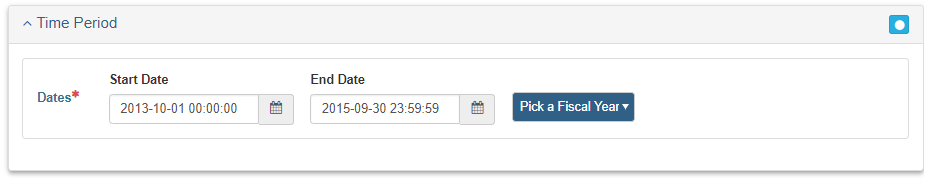
\includegraphics{images/main-time-period.png}

\hypertarget{project-metadata}{%
\section{Metadata Tab}\label{project-metadata}}

The Metadata tab describes your project's metadata, including a description that outlines the process of metadata creation, contributors to the creation of the metadata, and metadata repositories.

\begin{longtable}[]{@{}ll@{}}
\toprule
Quick Reference: Metadata Tab & Required?\tabularnewline
\midrule
\endhead
Basic Information: Metadata Status, Dates & Best Practice\tabularnewline
Metadata Contacts & Required\tabularnewline
Metadata Identifier & Required\tabularnewline
\bottomrule
\end{longtable}

\hypertarget{basic-information-1}{%
\subsection{Basic Information}\label{basic-information-1}}

\hypertarget{metadata-status-best-practice}{%
\subsubsection{Metadata Status (Best Practice)}\label{metadata-status-best-practice}}

Select the appropriate status of the creation of your metadata from the drop down menu. \emph{For example, if you have added all of your metadata, select ``completed.'' If you still have metadata to add, select ``onGoing.''}

\hypertarget{dates-best-practice-1}{%
\subsubsection{Dates (Best Practice)}\label{dates-best-practice-1}}

Add at least one date. Recommended are ``creation'' (when you first created your metadata) and ``lastUpdate'' (when you updated metadata after initial publication).

\hypertarget{metadata-contacts}{%
\subsection{Metadata Contacts}\label{metadata-contacts}}

Metadata Contacts are required. Adding a metadata contact will give users a contact point should they have any questions about the metadata.

\begin{longtable}[]{@{}lll@{}}
\toprule
Role & Contact & Required?\tabularnewline
\midrule
\endhead
author & Identified in Roles and Responsibilities & At least one is required\tabularnewline
pointOfContact & Identified in Roles and Responsibilities & Required\tabularnewline
\bottomrule
\end{longtable}

\hypertarget{metadata-identifier}{%
\subsection{Metadata Identifier}\label{metadata-identifier}}

The Metadata Identifier is automatically populated by mdEditor by generating a universally unique identifier (UUID). The metadata identifier gives each of your projects and products a unique ID and differentiates them from other similar projects and products.

\begin{rmdcaution}
Once a Metadata Identifier is created in the metadata, do not change it.
mdEditor uses the Metadata Identifier to connect records and changing
the Metadata Identifier can break those connections. If there are
additional identifiers you want to include in your metadata record,
include them in
\protect\hyperlink{project-main}{Main/Citation/Identifier}.
\end{rmdcaution}

\hypertarget{parent-metadata}{%
\subsection{Parent Metadata}\label{parent-metadata}}

{[}Under development{]}

\hypertarget{metadata-repositories}{%
\subsection{Metadata Repositories}\label{metadata-repositories}}

{[}Under development{]}

\begin{center}\rule{0.5\linewidth}{\linethickness}\end{center}

\hypertarget{project-keywords}{%
\section{Keyword Tab}\label{project-keywords}}

Adding keywords to your metadata record allows for the record to be found later through a search engine. Keywords are the way to tag your projects or products. The mdEditor is designed using thesauruses that contain pre-determined keywords.

\begin{longtable}[]{@{}ll@{}}
\toprule
Quick Reference: Keyword Tab & Required?\tabularnewline
\midrule
\endhead
ISO Topic Category & Required\tabularnewline
GCMD Keywords & Best Practice\tabularnewline
\bottomrule
\end{longtable}

\hypertarget{add-keywords-to-your-project}{%
\subsection{Add Keywords to your Project}\label{add-keywords-to-your-project}}

\begin{enumerate}
\def\labelenumi{\arabic{enumi}.}
\tightlist
\item
  Click ``+ Add Thesaurus'' on the right to add the different thesauruses.
\item
  From the drop down box, pick a thesaurus.
\item
  Add keywords from the following pre-populated thesauruses.
\item
  If none of the keywords in the following categories are sufficient for tagging your project, you can add other keywords with a custom thesaurus (see below for more information).
\end{enumerate}

\hypertarget{iso-topic-category-thesaurus-required}{%
\subsection{ISO Topic Category Thesaurus (Required)}\label{iso-topic-category-thesaurus-required}}

Because mdJSON metadata is based on the ISO (International Organization for Standardization) metadata standard, all projects must select at least one ISO Topic Category. ISO topics were generally meant for spatial data so they might be a bit of a stretch, but do your best to find the best fit. mdEditor provides definitions of each ISO topic category if you hover over the ? icon.

ISO Topic List:

\begin{enumerate}
\def\labelenumi{\arabic{enumi}.}
\tightlist
\item
  biota
\item
  boundaries
\item
  climatologyMeteorologyAtmosphere
\item
  economy
\item
  elevation
\item
  environment
\item
  geoscientificInformation
\item
  health
\item
  imageryBaseMapsEarthCover
\item
  intelligenceMilitary
\item
  inlandWaters
\item
  location
\item
  oceans
\item
  planningCadastre
\item
  society
\item
  structure
\item
  transportation
\item
  utilitiesCommunication
\end{enumerate}

\begin{rmdtip}
Biota and environment are probably the best fit for most AK-Region
projects.
\end{rmdtip}

\hypertarget{gcmd-keywords-thesaurus-best-practice}{%
\subsection{GCMD Keywords Thesaurus (Best Practice)}\label{gcmd-keywords-thesaurus-best-practice}}

GCMD stands for Global Change Master Directory and these keywords are maintained by NASA. Look for useful keywords in the GCMD Science Keywords. There are GCMD Platforms and Instruments Keywords but they are unlikely to apply to LCCs.

\begin{rmdtip}
Check the ``Full Path'' checkbox to save the full path of the keyword to
your metadata. This will maintain the category and context of the
specific keywords chosen.
\end{rmdtip}

\hypertarget{custom-thesaurus}{%
\subsection{Custom Thesaurus}\label{custom-thesaurus}}

If any of your desired keywords do not appear in the existing thesauruses, you can add them using a custom thesaurus. Use a custom thesaurus only for keywords that are not available in an existing thesaurus.

You cannot add keywords to an existing thesaurus; you can only add keywords in a custom thesaurus.

You cannot save a custom thesaurus in mdEditor.

\begin{rmdtip}
If you have a consistent set of keywords that you use across your
projects, you could add these to a ``template project'' record in
mdEditor and then modify the specific keywords you need for each
project. See the \protect\hyperlink{workflow}{workflow} section for more
info about using template records.
\end{rmdtip}

\hypertarget{keywords-and-sciencebase}{%
\subsection{Keywords and ScienceBase}\label{keywords-and-sciencebase}}

{[}Under development{]}

\begin{center}\rule{0.5\linewidth}{\linethickness}\end{center}

\hypertarget{project-extent}{%
\section{Extent Tab}\label{project-extent}}

\textbf{Extent} refers to geographic boundaries for your project. Spatial extents lets users see at a glance the geographic footprint of your project and allows searching within specific geographic areas.

\begin{longtable}[]{@{}ll@{}}
\toprule
Quick Reference: Extent Tab & Required?\tabularnewline
\midrule
\endhead
Extent & Required\tabularnewline
\bottomrule
\end{longtable}

\hypertarget{creating-extents}{%
\subsection{Creating Extents}\label{creating-extents}}

There are multiple ways to create a spatial extent for your project.

Clicking the \textbf{Edit Extent Features} button allows for the addition of \textbf{Feature Properties} such as: \textbf{ID}, \textbf{Name}, or \textbf{Description}. You can draw a polygon or a bounding box in the initial window.

You can export spatial extents and re-use for other records using the \textbf{import feature} button or by dragging and dropping onto the map.

Extents are limited to 5000 vertices. Recommend you create only simple polygons or bounding boxes. If you want greater detail, attach high-definition shapefiles instead of trying to draw them.

Extents should be accurate enough for searching purposes, but remember that they are metadata, not data.

\hypertarget{option-1-import-spatial-features}{%
\subsubsection{Option 1: Import Spatial Features}\label{option-1-import-spatial-features}}

Spatial features such as geoJSON, shapefiles, and kml can be imported. However, file attributes (such as name and description), will not be imported and must be added manually.

Important: coordinates used must be geographic coordinates, not projected coordinates.

\hypertarget{option-2-draw-spatial-features}{%
\subsubsection{Option 2: Draw Spatial Features}\label{option-2-draw-spatial-features}}

\begin{rmdtip}
It is easier to click ``finish'' when drawing a polygon instead of
trying to close the polygon by clicking on the first point.
\end{rmdtip}

\hypertarget{option-3-draw-bounding-box}{%
\subsubsection{Option 3: Draw Bounding Box}\label{option-3-draw-bounding-box}}

mdEditor can automatically calculate a bounding box if you have at least one extent in the metadata.

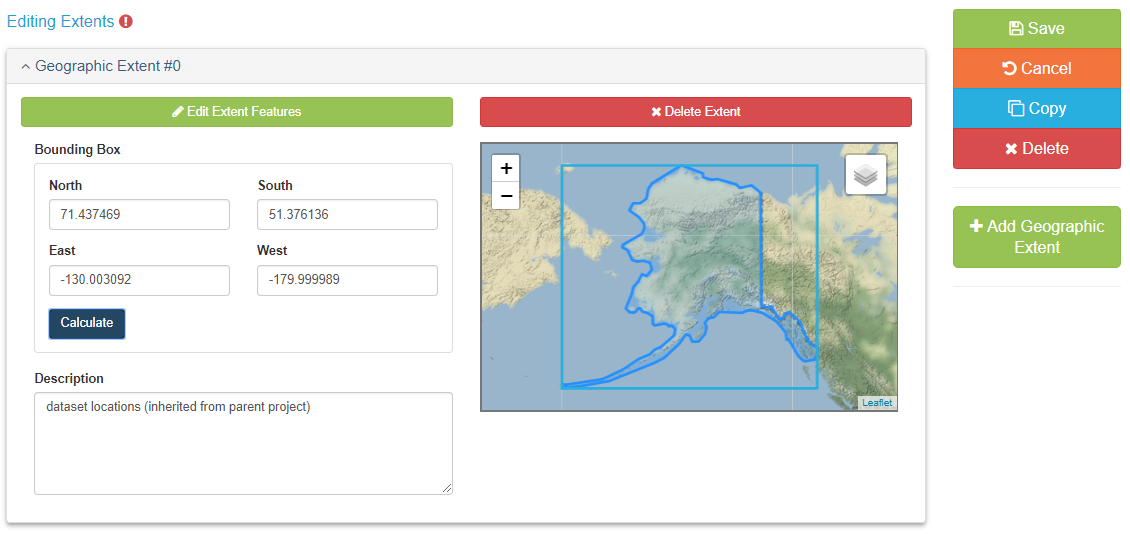
\includegraphics{images/extent_boundingbox-2.png}

Bounding boxes will not work across the dateline but you can have more than one extent per project. If your project area crosses the dateline, split the area into multiple extents and create separate bounding boxes.

\hypertarget{saving-and-exporting-extents}{%
\subsection{Saving and Exporting Extents}\label{saving-and-exporting-extents}}

\begin{rmdtip}
You can export, save, and import an extent to use for other projects or
products.
\end{rmdtip}

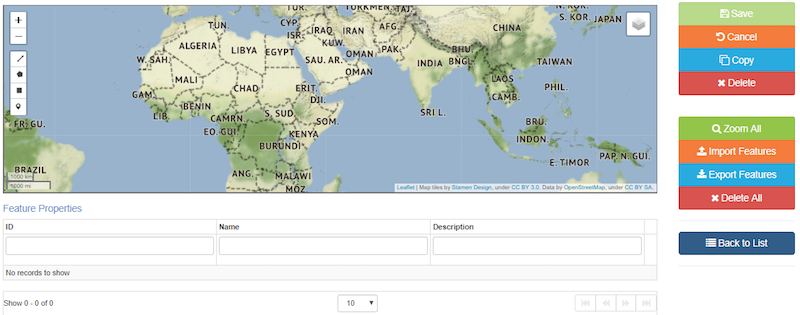
\includegraphics{images/edit_extent_page.png}

\hypertarget{project-taxonomy}{%
\section{Taxonomy Tab}\label{project-taxonomy}}

Taxonomy is required for projects and strongly recommended for products (where applicable).

\begin{longtable}[]{@{}ll@{}}
\toprule
Quick Reference: Taxonomy Tab & Required?\tabularnewline
\midrule
\endhead
Taxonomy & Required, if applicable\tabularnewline
\bottomrule
\end{longtable}

\hypertarget{taxonomy}{%
\subsection{Taxonomy}\label{taxonomy}}

mdEditor's new ``Taxonomy'' section automatically pulls in taxonomic information from ITIS (Integrated Taxonomic Information System -- see itis.gov for more information).

Please note that this functionality in mdEditor is not intended to explore ITIS. It is a tool to add known taxonomic information to your metadata. If you want to explore ITIS, go to itis.gov to find information and then come back to mdEditor with the desired search values.

The minimum requirements for valid taxonomy are a Taxonomic System plus one or more taxonomic classifications.

\hypertarget{add-taxonomic-system}{%
\subsubsection{Add Taxonomic System}\label{add-taxonomic-system}}

\begin{enumerate}
\def\labelenumi{\arabic{enumi}.}
\tightlist
\item
  Click ``Add Collection''
\end{enumerate}

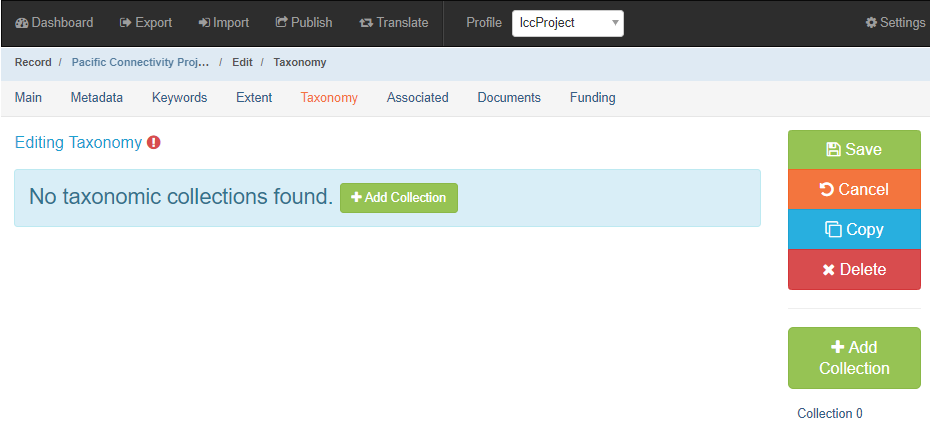
\includegraphics{images/taxonomy_addcollection.png}

\begin{enumerate}
\def\labelenumi{\arabic{enumi}.}
\setcounter{enumi}{1}
\tightlist
\item
  From here, you can click ``Add Taxa from ITIS'' directly (on right side) without adding the taxonomic system. This will be filled in for you automatically once you have added items from ITIS.
\end{enumerate}

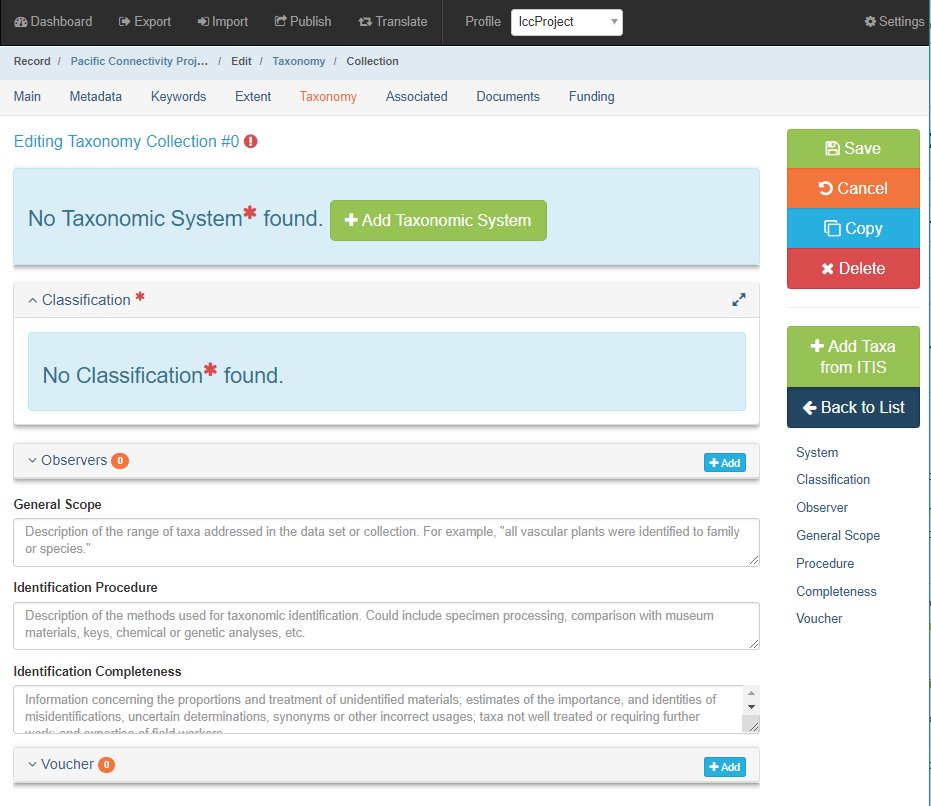
\includegraphics{images/taxonomy_addtaxafromitis.png}

\begin{enumerate}
\def\labelenumi{\arabic{enumi}.}
\setcounter{enumi}{2}
\tightlist
\item
  Enter your search terms in the search box. You can type in a common name, scientific name, or TSN (Taxonomic Serial Number, assigned by ITIS). You can type in any level of taxonomy, not just species name (e.g., you can type in an order or class or genus). You can specify by Kingdom if you like.
\end{enumerate}

If you haven't used the search in a while (or ever) the ITIS service might be asleep so it will take a few more seconds to load but then will load quickly after that.

The status of the taxonomic classification is denoted in () after the TSN. ITIS may consider a classification ``invalid'' if the species was reclassified, for example. It is up to you whether you want to add invalid ITIS classifications to your metadata.

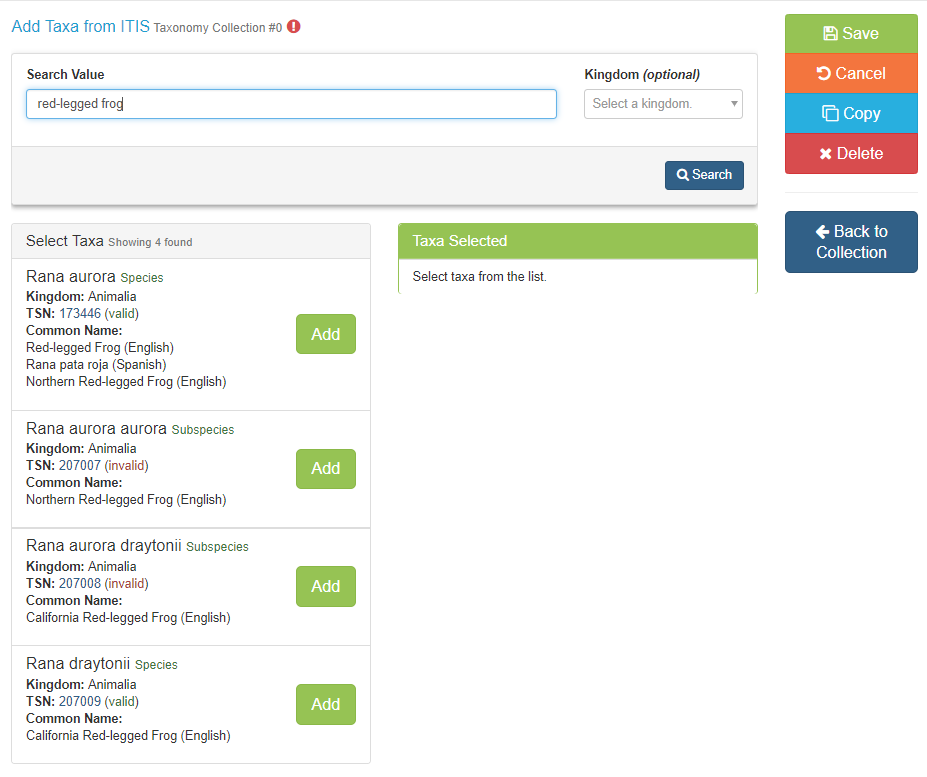
\includegraphics{images/taxonomy_search_redleggedfrog.png}

\begin{enumerate}
\def\labelenumi{\arabic{enumi}.}
\setcounter{enumi}{3}
\tightlist
\item
  Click ``Add'' for the search results you want to add to your record and then click ``Import Taxa.'' You will get a message of successful import at the bottom of your screen.
\end{enumerate}

You don't need to worry about clicking import multiple times for the same species. mdEditor is smart enough to know not to create duplicate entries of the same species.

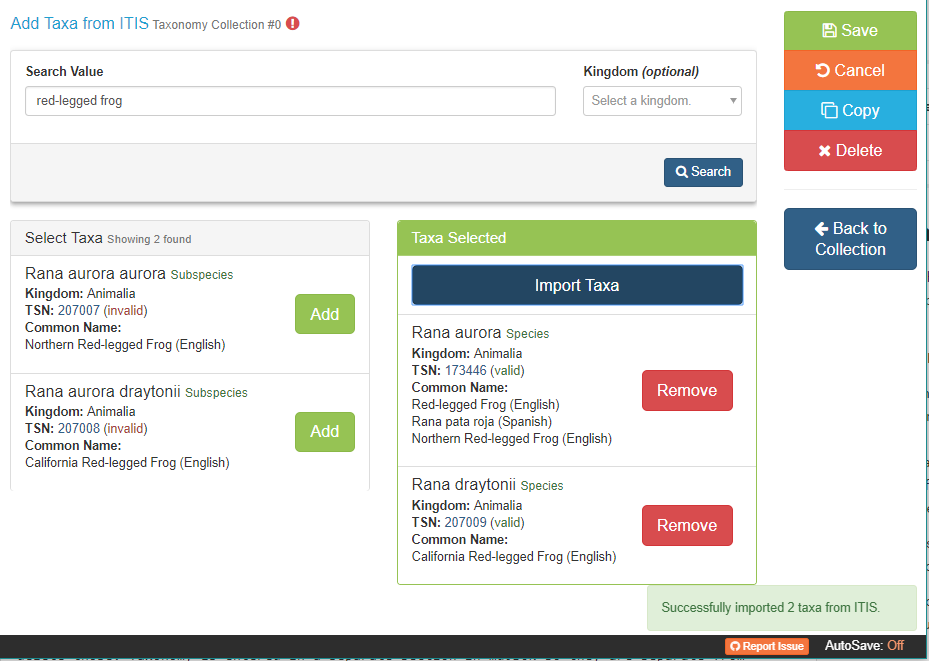
\includegraphics{images/taxonomy_successfulimport.png}

\begin{enumerate}
\def\labelenumi{\arabic{enumi}.}
\setcounter{enumi}{4}
\tightlist
\item
  Click ``Back to Collection.'' You will see that it has added a taxonomic hierarchy. It has also added a Title to Taxonomic System (if you hadn't already added one by hand). This completes the minimum information required for taxonomy.
\end{enumerate}

You can click on any level of the taxonomic hierarchy to collapse the entries below that level.

mdEditor only adds common names at the lowest taxonomic level you identified (e.g., species level).

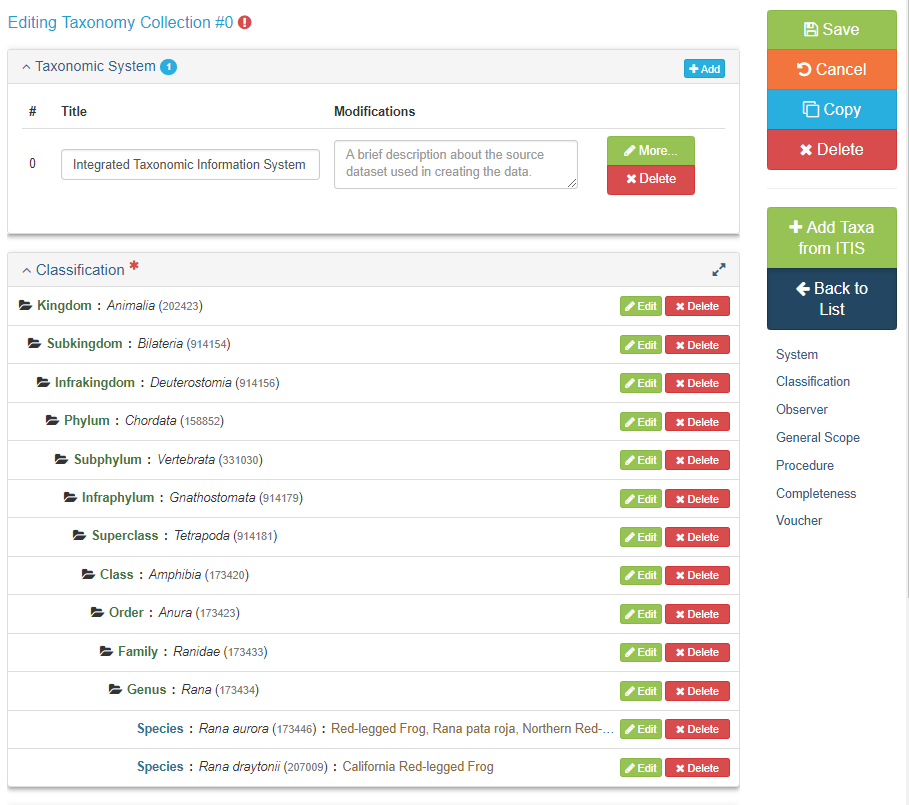
\includegraphics{images/taxonomy_collection.png}

\begin{enumerate}
\def\labelenumi{\arabic{enumi}.}
\setcounter{enumi}{5}
\tightlist
\item
  You can add additional information regarding the taxonomic information if you desire.
\end{enumerate}

\textbf{Observers} would be filled out when there were people who actually went in the field/lab and identified species. Here you would lie the people who did that work.

\begin{itemize}
\tightlist
\item
  General Scope: You can add a description of the range of taxa addressed in the dataset or collection.
\item
  Identification Procedure: You can describe the methods used for taxonomic identification.
\item
  Identification Completeness: You can add information regarding completeness and uncertainty in the identifications.
\end{itemize}

\textbf{Voucher} is where you can add information about specimens you submitted to a museum or a storage facility where you are storing specimens, can document that here (select a Repository via a Contact entered in mdEditor).

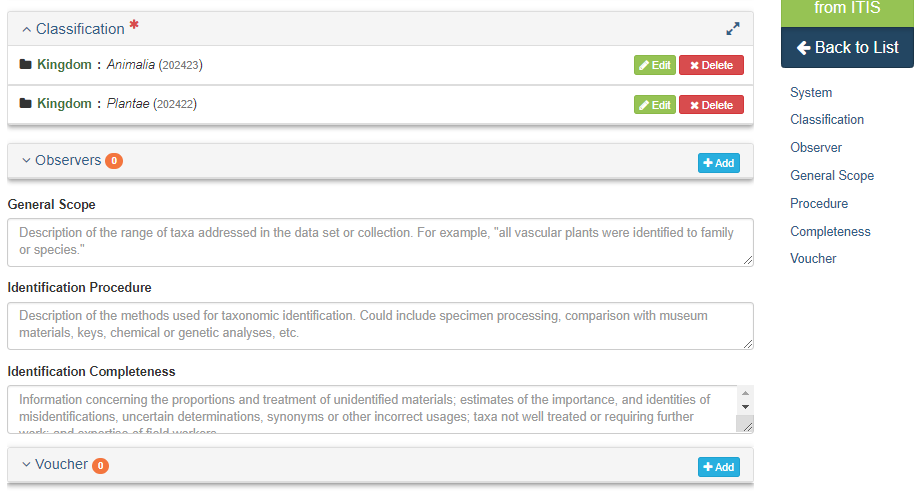
\includegraphics{images/taxonomy_additionalinfo.png}

\hypertarget{when-taxonomy-is-needed}{%
\subsection{When Taxonomy is Needed}\label{when-taxonomy-is-needed}}

Taxonomy is mostly used for search is discovery and functions similar to keywords.

If you have existing species names or other keywords, you do not need to delete those. Taxonomy is entered in a separate section in mdJSON so they are separate from Keywords.

To some extent, this is up to the judgement of the data manager. You will know best the connection of a resource to a specific species or other taxonomic group. For example, if a bear model was used to rank habitat for a prioritization product but the final output is not relevant to bears any longer, then you probably wouldn't want to add bear species in taxonomy.

\hypertarget{reporting-issues}{%
\subsection{Reporting Issues}\label{reporting-issues}}

If you encounter issues or bugs using the new Taxonomy feature, please report them in this github thread: \url{https://github.com/adiwg/mdEditor/issues/101} (requires github account to post).

\hypertarget{project-associations}{%
\section{Associated Tab}\label{project-associations}}

The Associated section is used to connect metadata records with each other. This feature should be used when items are related, for example, products are often the result of projects, and projects often have sub-projects. Projects and Products can be linked together by using association. Adding associations gives users the ability to find items that relate to each other.

\hypertarget{create-associations}{%
\subsection{Create Associations}\label{create-associations}}

In mdEditor you can either create the association from the Project record or the Product record. The ``Association Type'' will define the association from your current record to the linked record. Specifying the ``Linked Association Type'' will create the association from the other direction.

\begin{rmdwarning}
It is recommended you ALWAYS specify the Linked Association Type when
you create associations. This will ensure the associations are defined
from both directions and be present in the metadata no matter how the
metadata is translated or where it is used in the future.
\end{rmdwarning}

Associations can only be made after both project and product records have been created in mdEditor.

\begin{longtable}[]{@{}l@{}}
\toprule
\begin{minipage}[b]{0.97\columnwidth}\raggedright
\textbf{Quick Reference: Creating an Association in a Project Record}\strut
\end{minipage}\tabularnewline
\midrule
\endhead
\begin{minipage}[t]{0.97\columnwidth}\raggedright
1. Select ``product'' from the Association Type drop-down menu.\strut
\end{minipage}\tabularnewline
\begin{minipage}[t]{0.97\columnwidth}\raggedright
2. Use the Select a Record button to select an associated product.\strut
\end{minipage}\tabularnewline
\begin{minipage}[t]{0.97\columnwidth}\raggedright
3. Choose the product that you would like to associate from the ``Select a Resource'' list.\strut
\end{minipage}\tabularnewline
\begin{minipage}[t]{0.97\columnwidth}\raggedright
4. Fill out the Linked Association Type with ``parentProject.''\strut
\end{minipage}\tabularnewline
\bottomrule
\end{longtable}

\hypertarget{step-by-step-creating-an-association-in-a-project-record}{%
\subsubsection{Step-by-Step: Creating an Association in a Project Record}\label{step-by-step-creating-an-association-in-a-project-record}}

\textbf{Step 1}: Select ``\textbf{product}'' from the \textbf{Association Type} drop-down menu. This field will describe the relationship from the associated record to the project record (the associated record is the product of the project record you are editing).

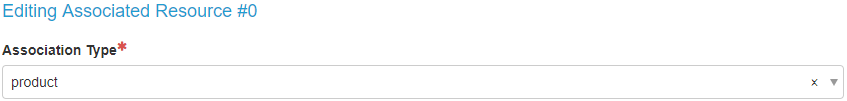
\includegraphics{images/product_association_lcc.png}

\textbf{Step 2}: Click the ``\textbf{Select a Record}'' button to select an associated product.

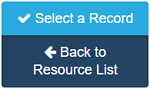
\includegraphics{images/select_a_record_button.png}

\textbf{Step 3}: Choose the product that you would like to associate from the \textbf{Select a Resource} list.

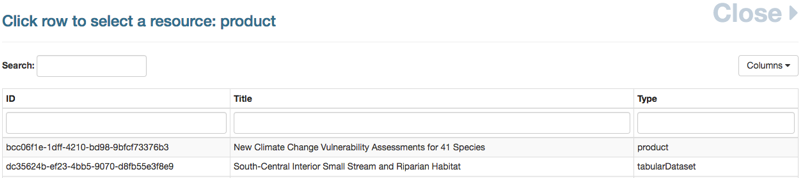
\includegraphics{images/select_a_resource_product_window.png}

\textbf{Step 4}: Fill out the Linked Association Type with ``\textbf{parentProject}.''

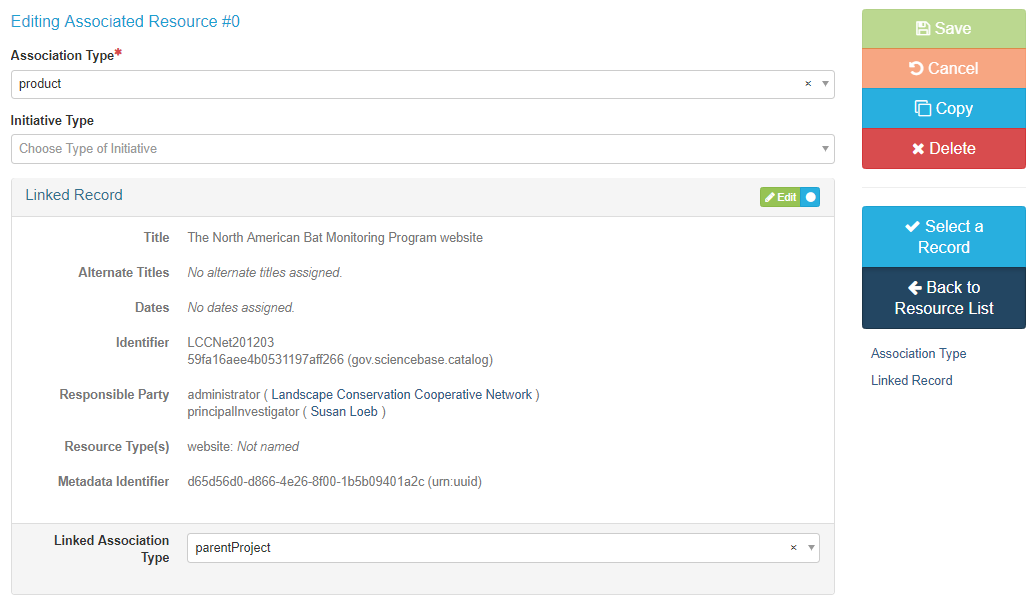
\includegraphics{images/project_association_linked_record.png}

\hypertarget{product-entry-guidance}{%
\chapter{Product Entry Guidance}\label{product-entry-guidance}}

The Product Entry Guidance section will cover how to create a metadata record for an AK-Region product.

\begin{center}\rule{0.5\linewidth}{\linethickness}\end{center}

\hypertarget{before-you-begin-1}{%
\section{Before You Begin}\label{before-you-begin-1}}

\hypertarget{select-the-lccproduct-profile}{%
\subsection{Select the lccProduct Profile:}\label{select-the-lccproduct-profile}}

After creating your product record and before you begin adding metadata, select \textbf{lccProduct} from the \textbf{Profile} drop down in the main menu. This will limit the number of available tabs and only show tabs that contain fields that are required for product creation.

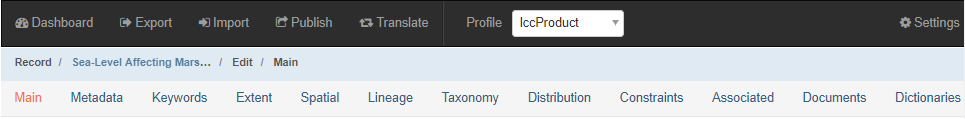
\includegraphics{images/profile_lccproduct.png}

\hypertarget{make-sure-your-contacts-are-loaded-into-mdeditor-1}{%
\subsection{\texorpdfstring{Make sure your \protect\hyperlink{contact-entry_guidance}{contacts} are loaded into mdEditor:}{Make sure your contacts are loaded into mdEditor:}}\label{make-sure-your-contacts-are-loaded-into-mdeditor-1}}

In mdEditor, contacts are created separately from individual records, and then stored within a library in mdEditor. Once contacts have been entered or imported into mdEditor, they can be used in metadata records.

You should maintain a single list of your contacts in the program's archive folder (root folder that contains all project archive folders). Having duplicate copies of the same contact is not desirable. It can create confusion as you edit and manage your metadata records and introduce unnecessary errors.

\begin{center}\rule{0.5\linewidth}{\linethickness}\end{center}

\hypertarget{edit-a-product}{%
\section{Edit a Product}\label{edit-a-product}}

\begin{enumerate}
\def\labelenumi{\arabic{enumi}.}
\tightlist
\item
  Import or create your product record (see \protect\hyperlink{workflow}{workflow}).
\item
  Choose the specific Resource Type that describes your product. Do not choose the generic ``product.''
\item
  Select the lccProduct Profile: from the Main Menu (Top Navigation Bar) select ``lccProduct'' from the profile drop-down menu.
\item
  Fill out metadata information for the following tabs:
\end{enumerate}

\begin{itemize}
\tightlist
\item
  \protect\hyperlink{product-main}{Main Tab}
\item
  \protect\hyperlink{product-metadata}{Metadata Tab}
\item
  \protect\hyperlink{product-keywords}{Keywords Tab}
\item
  \protect\hyperlink{product-extent}{Extent Tab}
\item
  \protect\hyperlink{product-taxonomy}{Taxonomy Tab}
\item
  \protect\hyperlink{product-lineage}{Lineage Tab}
\item
  \protect\hyperlink{product-distribution}{Distribution Tab}
\item
  \protect\hyperlink{product-constaints}{Constraints Tab}
\item
  \protect\hyperlink{product-dictionary}{Dictionaries Tab}
\end{itemize}

\begin{enumerate}
\def\labelenumi{\arabic{enumi}.}
\setcounter{enumi}{4}
\tightlist
\item
  If applicable, \protect\hyperlink{product-associated}{associate} your products with other metadata records.
\end{enumerate}

\begin{center}\rule{0.5\linewidth}{\linethickness}\end{center}

\hypertarget{required-fields-for-products}{%
\section{Required Fields for Products}\label{required-fields-for-products}}

\hypertarget{main-tab-2}{%
\subsection{Main Tab}\label{main-tab-2}}

\begin{itemize}
\tightlist
\item
  Title
\item
  Status
\item
  Language
\item
  Resource Type
\item
  Point of Contact
\item
  Main Citation

  \begin{itemize}
  \tightlist
  \item
    Identifier
  \item
    Online Resource URL
  \item
    Responsible Parties
  \end{itemize}
\item
  Description

  \begin{itemize}
  \tightlist
  \item
    Abstract
  \end{itemize}
\item
  Time Period

  \begin{itemize}
  \tightlist
  \item
    Start Date
  \item
    End Date
  \end{itemize}
\end{itemize}

\hypertarget{metadata-tab-1}{%
\subsection{Metadata Tab}\label{metadata-tab-1}}

\begin{itemize}
\tightlist
\item
  Metadata Contacts
\item
  Metadata Identifier
\end{itemize}

\hypertarget{keywords-tab-1}{%
\subsection{Keywords Tab}\label{keywords-tab-1}}

\begin{itemize}
\tightlist
\item
  ISO Topic Category
\item
  GCMD Keywords (Best Practice)
\end{itemize}

\hypertarget{extent-tab-1}{%
\subsection{Extent Tab}\label{extent-tab-1}}

\begin{itemize}
\tightlist
\item
  Geographic Extent
\end{itemize}

\hypertarget{taxonomy-tab-1}{%
\subsection{Taxonomy Tab}\label{taxonomy-tab-1}}

\begin{itemize}
\tightlist
\item
  Taxonomic classifications
\end{itemize}

\hypertarget{distribution-tab}{%
\subsection{Distribution Tab}\label{distribution-tab}}

\begin{itemize}
\tightlist
\item
  Distributor

  \begin{itemize}
  \tightlist
  \item
    Contact
  \item
    Role
  \item
    Online Option

    \begin{itemize}
    \tightlist
    \item
      URL
    \end{itemize}
  \end{itemize}
\end{itemize}

\begin{center}\rule{0.5\linewidth}{\linethickness}\end{center}

\hypertarget{product-main}{%
\section{Main Tab}\label{product-main}}

The Main tab allows for the creation and/or editing of primary metadata.

\begin{longtable}[]{@{}ll@{}}
\toprule
Quick Reference: Product Main Tab & Required?\tabularnewline
\midrule
\endhead
Basic Information: Title, Status & Required\tabularnewline
Resource Type & Required\tabularnewline
Point of Contact & Required\tabularnewline
Citation: Title, Responsible Parties, Online Resource & Required\tabularnewline
Citation: Alternative Titles, Date & Optional\tabularnewline
Description: Abstact & Required\tabularnewline
Time Period: Start Date, End Date & Required\tabularnewline
\bottomrule
\end{longtable}

\hypertarget{basic-information-2}{%
\subsection{Basic Information}\label{basic-information-2}}

\hypertarget{record-id-required}{%
\subsubsection{Record ID (Required)}\label{record-id-required}}

Will be auto-generated but can be edited.

\hypertarget{title-required-1}{%
\subsubsection{Title (Required)}\label{title-required-1}}

Enter as informative a title as possible. Good titles, when they appear in a search, will be understood and/or traceable.

\hypertarget{status-required-1}{%
\subsubsection{Status (Required)}\label{status-required-1}}

The Status drop-down menu allows you to select the status of your product. Choose status ONLY from the four following options: \emph{completed, ongoing, proposed, or accepted}.

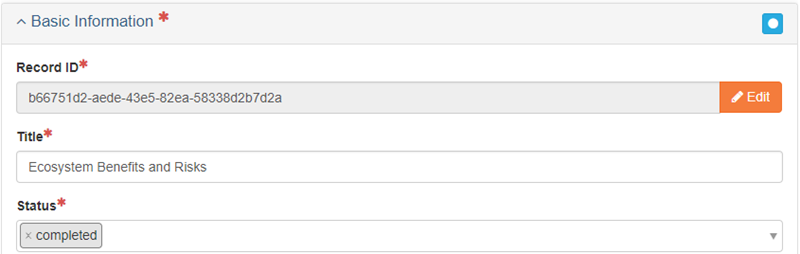
\includegraphics{images/main_screenshot_updated.png}

\hypertarget{default-locale-1}{%
\subsection{Default Locale}\label{default-locale-1}}

\textbf{Default Locale} allows for the selection of \textbf{Language}, \textbf{Character Set}, and \textbf{Country}. English, UTF-8, and USA will be selected by default, but you may change them if necessary.

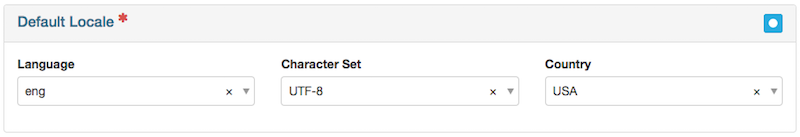
\includegraphics{images/default_locale.png}

\hypertarget{resource-types-required-1}{%
\subsection{Resource Types (Required)}\label{resource-types-required-1}}

The Resource Type should be automatically filled in with the resource type you selected when you created your record. Name is optional - you can leave this blank.

Products must have a specific resource type selected (not just ``product'').

\hypertarget{points-of-contact-required}{%
\subsection{Points of Contact (Required)}\label{points-of-contact-required}}

Adding a point of contact gives users information on who to contact should they have a question regarding your project or product.

\begin{rmdtip}
To add contacts to a metadata record, you must first create/upload the
contacts into mdEditor. See the Contact Section for more information.
\end{rmdtip}

\hypertarget{contacts-2}{%
\subsubsection{Contacts}\label{contacts-2}}

\begin{longtable}[]{@{}lll@{}}
\toprule
Role & Contact & Required?\tabularnewline
\midrule
\endhead
pointOfContact & Identified in Roles and Responsibilities & Required\tabularnewline
principalInvestigator & The Project PI & Best Practice\tabularnewline
\bottomrule
\end{longtable}

The point of contact for a project should be identified with Roles and Responsibilities (see Interim DM Implementation Guide). This is an interim solution as the point of contact can become obsolete if there is a positional change within an organization.

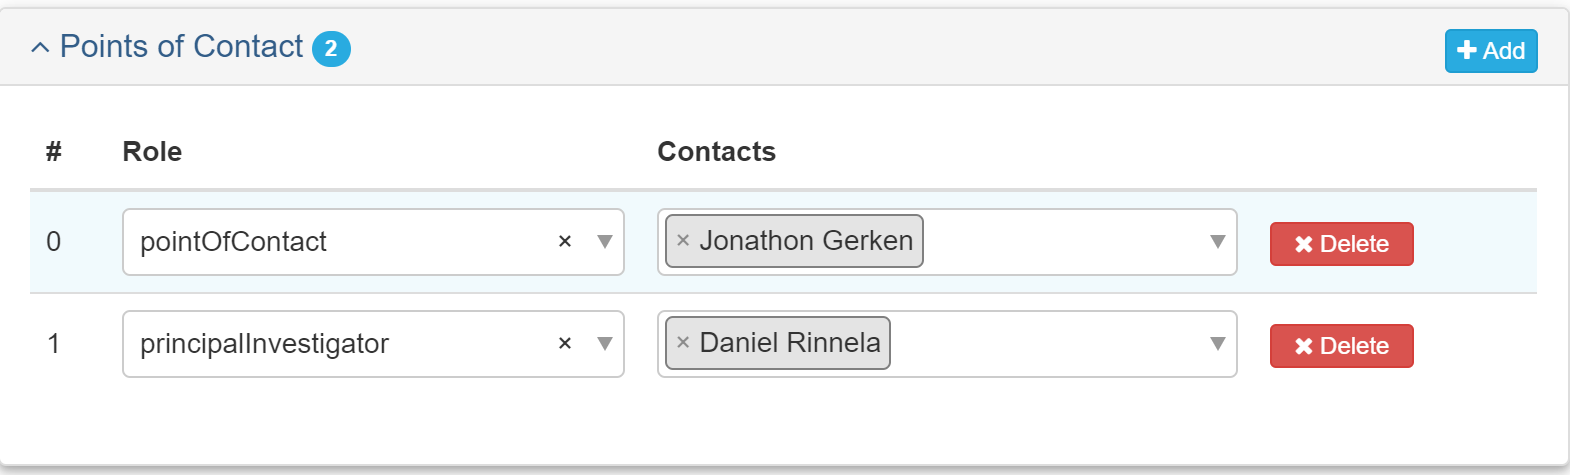
\includegraphics{images/7H_image.png}

\hypertarget{citation-1}{%
\subsection{Citation}\label{citation-1}}

The \textbf{Citation} describes pertinent information about your project such as: responsible parties, internal identifiers, and any online resources that may relate to your item. Adding information in the citation will also improve users' ability to find your items.

\hypertarget{citation-required-fields-1}{%
\subsubsection{Citation Required Fields}\label{citation-required-fields-1}}

\hypertarget{title-required-2}{%
\paragraph{Title (Required)}\label{title-required-2}}

The citation title is automatically populated with the title of your record.

\hypertarget{alternate-title-optional}{%
\paragraph{Alternate Title (Optional)}\label{alternate-title-optional}}

You can add an alternate title if desired, such as the Short Title used in the archive record.

\hypertarget{dates-optional}{%
\paragraph{Dates (Optional)}\label{dates-optional}}

Enter \emph{acquisition, creation, revision}, or another date reference from the picklist and then enter the date.

\hypertarget{responsible-parties-required-1}{%
\paragraph{Responsible Parties (Required)}\label{responsible-parties-required-1}}

Responsible parties must include a point of contact, but may also include the other responsible parties identified in Roles and Responsibilities (see Interim DM Implementation Guide) such as custodian, editor (data steward), and administrator.

\begin{rmdtip}
To add contacts to a metadata record, you must first create/upload the
contacts into mdEditor. See the Contact Section for more information.
\end{rmdtip}

\begin{longtable}[]{@{}lll@{}}
\toprule
Role & Contact & Required?\tabularnewline
\midrule
\endhead
pointOfContact & Identified in Roles and Responsibilities & Required\tabularnewline
custodian & Best Practice &\tabularnewline
editor & Best Practice &\tabularnewline
administrator & Best Practice &\tabularnewline
\bottomrule
\end{longtable}

\hypertarget{online-resource-required-if-available}{%
\paragraph{Online Resource (Required, if available)}\label{online-resource-required-if-available}}

Enter the Name and URL for the project homepage, if available.

\begin{rmdcaution}
If the product metadata was created by copying another mdEditor metadata
record, this identifier needs to be edited/changed since it will reflect
the copied record identifier. Only the mdEditor UUID changes to
represent a new record when an item is copied. Consult the
\protect\hyperlink{copy-records}{Copy Records} section of this manual to
learn how to make a copy.
\end{rmdcaution}

\hypertarget{description-1}{%
\subsection{Description}\label{description-1}}

Description allows for the addition of the Abstract as well as a Short Abstract, and Supplemental Information.

\hypertarget{abstract-required-1}{%
\subsubsection{Abstract (Required)}\label{abstract-required-1}}

Enter an abstract that succinctly describes the project's purpose and goals. Include key species or habitats as well.

\begin{rmdtip}
Write your project abstract in the present tense if the project is in
progress and past tense if the project has been completed.
\end{rmdtip}

\hypertarget{short-abstract-optional-1}{%
\subsubsection{Short Abstract (Optional)}\label{short-abstract-optional-1}}

Enter a short description, limited to 300 characters, if desired.

Enter comments, if desired.

\hypertarget{time-period-1}{%
\subsection{Time Period}\label{time-period-1}}

\textbf{Time Period} refers to project start and end date, or the date that the product was applicable (e.g., time that a map is valid, date of publication, date of presentation).

\textbf{Required}: For each product, add a start date and end date.

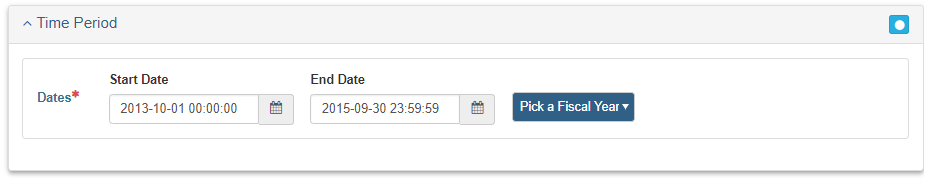
\includegraphics{images/main-time-period.png}

\begin{center}\rule{0.5\linewidth}{\linethickness}\end{center}

\hypertarget{product-metadata}{%
\section{Metadata Tab}\label{product-metadata}}

Record Metadata includes a description that outlines the process of metadata creation, contributors to the creation of the metadata, and metadata repositories.

\begin{longtable}[]{@{}ll@{}}
\toprule
Quick Reference: Product Metadata Tab & Required?\tabularnewline
\midrule
\endhead
Basic Information & Required\tabularnewline
Metadata Contacts & Required\tabularnewline
Metadata Identifier & Required\tabularnewline
\bottomrule
\end{longtable}

\hypertarget{basic-information-3}{%
\subsection{Basic Information}\label{basic-information-3}}

\hypertarget{metadata-status-best-practice-1}{%
\subsubsection{Metadata Status (Best Practice)}\label{metadata-status-best-practice-1}}

Select the appropriate status of the creation of your metadata from the drop down menu. For example, if you have added all of your metadata, select ``completed.'' If you still have metadata to add, select ``onGoing.''

\hypertarget{dates-best-practice-2}{%
\subsubsection{Dates (Best Practice)}\label{dates-best-practice-2}}

Add at least one date. Recommended are ``creation'' (when you first created your metadata) and ``lastUpdate'' (when you updated metadata after initial publication).

\hypertarget{metadata-contacts-1}{%
\subsection{Metadata Contacts}\label{metadata-contacts-1}}

Metadata Contacts are required. Adding a metadata contact will give users a contact point should they have any questions about the metadata.

\begin{longtable}[]{@{}lll@{}}
\toprule
Role & Contact & Required?\tabularnewline
\midrule
\endhead
author & Identified in Roles and Responsibilities & At least one is required\tabularnewline
pointOfContact & Identified in Roles and Responsibilities & Required\tabularnewline
\bottomrule
\end{longtable}

\hypertarget{metadata-identifier-1}{%
\subsection{Metadata Identifier}\label{metadata-identifier-1}}

The Metadata Identifier is automatically populated by mdEditor by generating a universally unique identifier (UUID). The metadata identifier gives each of your projects and products a unique ID and differentiates them from other similar projects and products.

\begin{rmdwarning}
Once a Metadata Identifier is created in the metadata, do not change it.
mdEditor uses the Metadata Identifier to connect records and changing
the Metadata Identifier can break those connections. If there are
additional identifiers you want to include in your metadata record,
include them in Main/Citation/Identifier.
\end{rmdwarning}

\hypertarget{parent-metadata-1}{%
\subsection{Parent Metadata}\label{parent-metadata-1}}

{[}Under development{]}

\hypertarget{metadata-repositories-1}{%
\subsection{Metadata Repositories}\label{metadata-repositories-1}}

{[}Under development{]}

\begin{center}\rule{0.5\linewidth}{\linethickness}\end{center}

\hypertarget{product-keywords}{%
\section{Keyword Tab}\label{product-keywords}}

Adding keywords to your metadata record allows for the record to be found later through a search engine. Keywords are the way to tag your projects or products. The mdEditor is designed using thesauruses that contain pre-determined keywords.

\begin{longtable}[]{@{}ll@{}}
\toprule
Quick Reference: Product Keywords Tab & Required?\tabularnewline
\midrule
\endhead
ISO Topic Category & Required\tabularnewline
GCMD Keywords & Required\tabularnewline
\bottomrule
\end{longtable}

\hypertarget{add-keywords-to-your-product-record}{%
\subsection{Add Keywords to your Product Record}\label{add-keywords-to-your-product-record}}

\begin{enumerate}
\def\labelenumi{\arabic{enumi}.}
\tightlist
\item
  Click ``+ Add Thesaurus'' on the right to add the different thesauruses.
\item
  From the drop down box, pick a thesaurus.
\item
  Add keywords from the following pre-populated thesauruses.
\item
  If none of the keywords in the following categories are sufficient for tagging your project, you can add other keywords with a custom thesaurus (see below for more information).
\end{enumerate}

\hypertarget{iso-topic-category-thesaurus-required-1}{%
\subsection{ISO Topic Category Thesaurus (Required)}\label{iso-topic-category-thesaurus-required-1}}

Because mdJSON metadata is based on the ISO (International Organization for Standardization) metadata standard, all products must select at least one ISO Topic Category. ISO topics were generally meant for spatial data so they might be a bit of a stretch, but do your best to find the best fit. mdEditor provides definitions of each ISO topic category if you hover over the ? icon.

ISO Topic List:
1. biota
2. boundaries
3. climatologyMeteorologyAtmosphere
4. economy
5. elevation
6. environment
7. geoscientificInformation
8. health
9. imageryBaseMapsEarthCover
10. intelligenceMilitary
11. inlandWaters
12. location
13. oceans
14. planningCadastre
15. society
16. structure
17.transportation
18 utilitiesCommunication

\begin{rmdtip}
Biota and environment are probably the best fit for most AK-Region
products.
\end{rmdtip}

\hypertarget{gcmd-keywords-thesaurus-best-practice-1}{%
\subsection{GCMD Keywords Thesaurus (Best Practice)}\label{gcmd-keywords-thesaurus-best-practice-1}}

GCMD stands for Global Change Master Directory and these keywords are maintained by NASA. Look for useful keywords in the GCMD Science Keywords. There are GCMD Platforms and Instruments Keywords but they are unlikely to apply to LCCs.

\begin{rmdtip}
Check the ``Full Path'' checkbox to save the full path of the keyword to
your metadata. This will maintain the category and context of the
specific keywords chosen.
\end{rmdtip}

\hypertarget{custom-thesaurus-1}{%
\subsection{Custom Thesaurus}\label{custom-thesaurus-1}}

If any of your desired keywords do not appear in the existing thesauruses, you can add them using a custom thesaurus. Use a custom thesaurus only for keywords that are not available in an existing thesaurus.

You cannot add keywords to an existing thesaurus; you can only add keywords in a custom thesaurus.

You cannot save a custom thesaurus in mdEditor.

\begin{rmdtip}
If you have a consistent set of keywords that you use across your
products, you could add these to a ``template product'' record in
mdEditor and then modify the specific keywords you need for each
product. See the workflow section for more info about using template
records.
\end{rmdtip}

\hypertarget{keywords-and-sciencebase-1}{%
\subsection{Keywords and ScienceBase}\label{keywords-and-sciencebase-1}}

{[} Under development {]}

\begin{center}\rule{0.5\linewidth}{\linethickness}\end{center}

\hypertarget{product-extent}{%
\section{Extent Tab}\label{product-extent}}

\textbf{Extent} refers to geographic boundaries for your project. Spatial extents lets users see at a glance the geographic footprint of your project and allows searching within specific geographic areas.

\begin{longtable}[]{@{}ll@{}}
\toprule
Quick Reference: Product Extent Tab & Required?\tabularnewline
\midrule
\endhead
Extent & Required\tabularnewline
\bottomrule
\end{longtable}

Spatial extents should be included for all applicable products. As a default, products can inherit extents from their parent project.

\begin{rmdtip}
You can export, save, and import an extent to use for other projects or
products.
\end{rmdtip}

See further information on Extents in \protect\hyperlink{project-extent}{Project Extent entry guidance}.

\begin{center}\rule{0.5\linewidth}{\linethickness}\end{center}

\hypertarget{product-taxonomy}{%
\section{Taxonomy Tab}\label{product-taxonomy}}

\begin{longtable}[]{@{}ll@{}}
\toprule
Quick Reference: Product Taxonomy Tab & Required?\tabularnewline
\midrule
\endhead
Taxonomy & Required\tabularnewline
\bottomrule
\end{longtable}

Please see the \protect\hyperlink{project-taxonomy}{Project Taxonomy entry guidance section}.

Taxonomy is required for projects and strongly recommended for products (where applicable).

\begin{center}\rule{0.5\linewidth}{\linethickness}\end{center}

\hypertarget{product-lineage}{%
\section{Lineage Tab}\label{product-lineage}}

Lineage is used to track the process of building spatial datasets. It's a space that can be used to describe the steps and sources used to create the product, and document the roles and contacts for the product contributors. Completing the lineage tab is recommended, but not required.

\begin{itemize}
\tightlist
\item
  \textbf{Statement} (Required): Notes actions taken to verify, transform, repair, and integrate the resource.
\item
  \textbf{Process Step} (Optional): Consult the Process Step section below to learn how to add information about the creation of your project.
  -\textbf{Sources} (Optional): Use the Sources field to indicate what you used to create the product and then write a statement. This can be done instead of completing all other fields in this tab.
  -\textbf{Citation} (Optional): If you have a citation for a manual, enter it here. This can be done instead of completing all other fields in this tab.
  -\textbf{Scope} (Optional): Select type from the picklist.
\end{itemize}

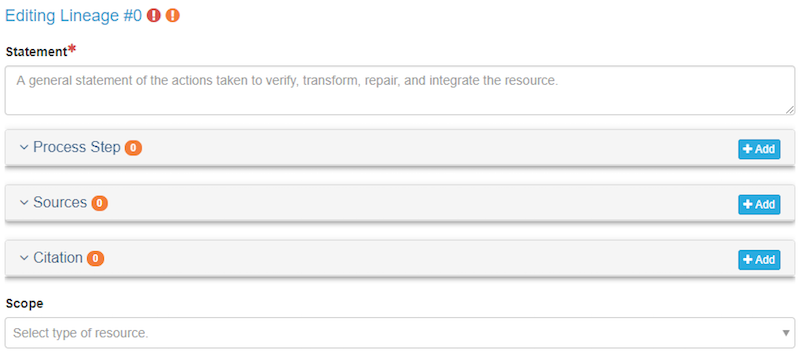
\includegraphics{images/lineage_window.png}

\hypertarget{process-step}{%
\subsection{Process Step}\label{process-step}}

\textbf{Process Step} allows for documentation of the steps taken to build spatial data.

\emph{The following are available and required:}
-Step ID: (Auto filled depending on the number of Process Steps added).
-Description: Add a description of the process step.

\emph{The following fields are available but optional:}
-\textbf{Step Sources}: Information about the source data used in the process step.
-\textbf{Step Products}: Information about an intermediate data set.
-\textbf{Processors}: Processors of the process step.
+ Select or enter a role from the \textbf{Role} drop-down and select a contact from the \textbf{Contacts} drop down.
+ Consult the \protect\hyperlink{contacts}{Contacts} section of this manual to learn about adding contacts.
- \textbf{Step Reference}: Add a citation noting your step process references.
- \textbf{Time Period}: Add a time period noting the \textbf{Start Date, End Date}, and \textbf{Fiscal Year}.
+ \textbf{ID}: Add a unique identifier for the time period.
+ \textbf{Description}: Add a description of the time period.
+ \textbf{Time Period Name}: Add a name for your time period.
+ \textbf{Interval}: Enter an \textbf{Interval Amount} and \textbf{Time Unit} of the time period.
+ \textbf{Duration}: Describe the time period in terms of \textbf{Years, Months, Days, Hours, Minutes}, and \textbf{Seconds}.
- Scope: Select the type of resource from the drop-down menu.

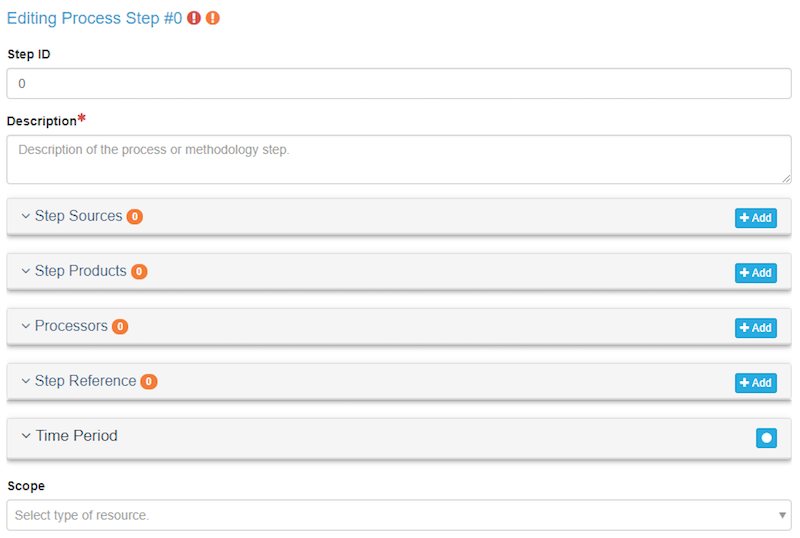
\includegraphics{images/process_step_window.png}

\begin{center}\rule{0.5\linewidth}{\linethickness}\end{center}

\hypertarget{product-distribution}{%
\section{Distribution Tab}\label{product-distribution}}

\textbf{Distribution} provides documentation on how or where users can obtain products. Distribution methods may include online options (e.g., website, database) or offline options (e.g., delivery via mail, library).

An online distribution link is required for any products sent to data.gov.

\begin{longtable}[]{@{}ll@{}}
\toprule
Quick Reference: Product Distribution Tab & Required?\tabularnewline
\midrule
\endhead
Contacts and Role & Required\tabularnewline
Transfer Options: Online Option & Required\tabularnewline
\bottomrule
\end{longtable}

Click \textbf{Add Distribution Section} and then \textbf{Edit Distributors} to begin adding distributors.

\hypertarget{distributor}{%
\subsection{Distributor}\label{distributor}}

This section involves adding distributor information and a URL for data products that are hosted anywhere. For example, if The Nature Conservancy is hosting a data source, the distributor is ``The Nature Conservancy.''

\hypertarget{contacts-and-role-required}{%
\subsubsection{Contacts and Role (Required)}\label{contacts-and-role-required}}

If anything is filled out in the distribution section, a contact must be added. The appropriate role is ``distributor.''

The contact should ideally be someone who will remain available to respond to potential inquiries about the product.

\hypertarget{transfer-options-required}{%
\subsection{Transfer Options (Required)}\label{transfer-options-required}}

Transfer Options provide details regarding obtaining the product. Online and offline options are available.

\hypertarget{online-option-required-if-available}{%
\subsubsection{Online Option (Required if Available)}\label{online-option-required-if-available}}

\textbf{Name}
The Name of the online resource should be something that indicates it is a product page where the data can be downloaded. Examples: ``product webpage'' or ``Product Webpage with Downloadable Files.'' If there are multiple files for a single product record, the Name should be different for each file so the user can differentiate between them. For example, ``Download Aguiguan Veg 2016 data'' or ``Download FDM Veg 2011 data.''

Unique Names for multiple files are particularly important for items being sent to data.gov. Without a name specified at all, the link will display as ``webpage,'' which isn't particularly informative to users. Identical names for different files also won't be particularly informative.

\textbf{URL}
The most important thing to enter is the URL where the product can be accessed or downloaded.
An online link is required for any products sent to data.gov. Preferably the link should be a direct download to the data and not an intermediary page.

\textbf{Function}
In the Function field, you should indicate the type of URL. If the link is a direct download of the data, select ``download.'' If the link goes to an informational page, select ``information.''

\textbf{How to obtain download link from ScienceBase Items}
{[}Under development{]}

\textbf{Offline Option}
If your product is only available offline, describe how users can obtain the product here.

\hypertarget{example-distributor}{%
\subsection{Example Distributor}\label{example-distributor}}

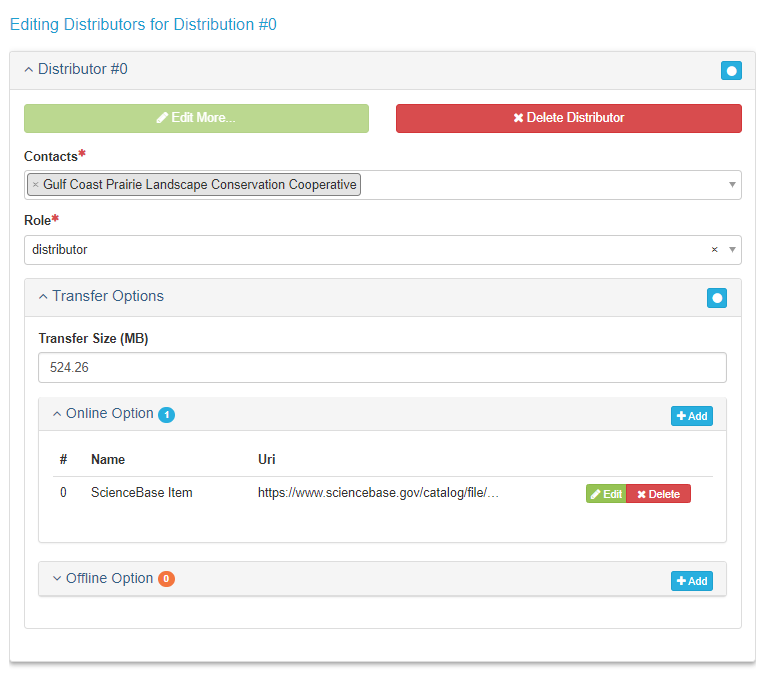
\includegraphics{images/distribution_example.png}

\begin{center}\rule{0.5\linewidth}{\linethickness}\end{center}

\hypertarget{product-constraints}{%
\section{Constraints Tab}\label{product-constraints}}

The Constraint tab allows you to enter information into the metadata about how the resource can and cannot be used.

\begin{longtable}[]{@{}ll@{}}
\toprule
Quick Reference: Product Contraints Tab & Required?\tabularnewline
\midrule
\endhead
Use Limitation & Optional\tabularnewline
Legal & Optional\tabularnewline
Security Constaints & Optional\tabularnewline
\bottomrule
\end{longtable}

\hypertarget{use-limitation}{%
\subsection{Use Limitation}\label{use-limitation}}

Identify concerns over how people should or should not use the product.

If your product is licensed, let people know here. Typically files used will be public domain, but not always.

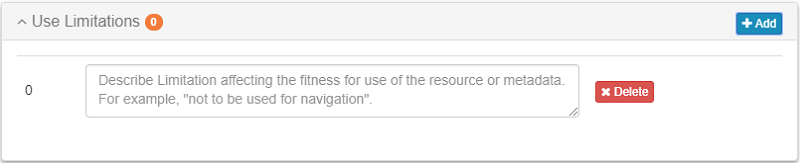
\includegraphics{images/use_limitation.png}

\hypertarget{legal}{%
\subsection{Legal}\label{legal}}

\begin{itemize}
\tightlist
\item
  \textbf{Access Constraints}: Access constraints are applied to assure the protection of privacy or intellectual property and any special restrictions or limitations on obtaining the resource.
\item
  \textbf{Use constraints}: How the product should be used.
\item
  \textbf{Other constraints}: This is a place to put standard disclaimers.
\end{itemize}

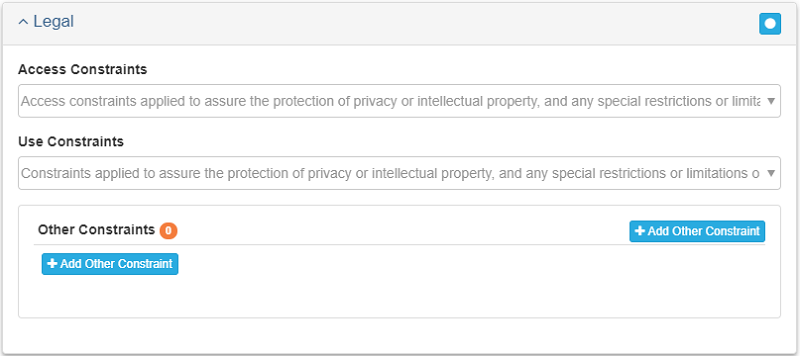
\includegraphics{images/legal.png}

\hypertarget{security-constraints}{%
\subsection{Security Constraints}\label{security-constraints}}

A place to describe constraints or restrictions pertaining to security of the resource. Choose classification from the drop-down menu.

Classification is the class of security (e.g., top secret, public access).

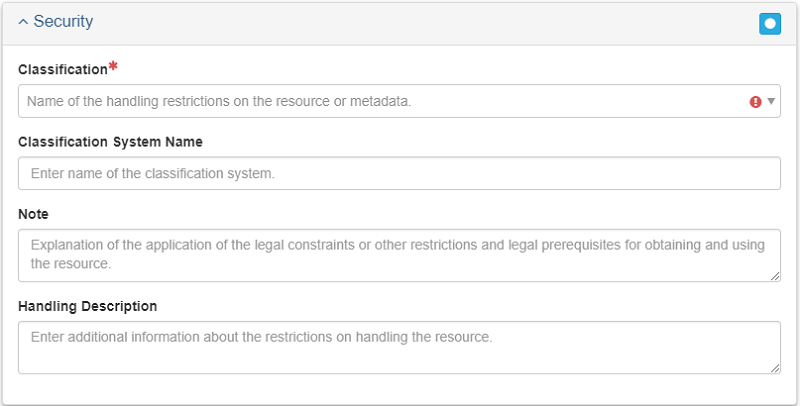
\includegraphics{images/security.png}

\begin{center}\rule{0.5\linewidth}{\linethickness}\end{center}

\hypertarget{product-dictionary}{%
\section{Dictionaries Tab}\label{product-dictionary}}

Data dictionaries are required for tabular datasets.

Like Contacts, data dictionaries are created separately from Product records. Also like Contacts, Dictionaries can be reused across products and are stored outside the project archive folder in the program archive folder. See \protect\hyperlink{dictionary-entry-guidance}{Dictionary Entry Guidance} for details. The Dictionaries tab links the product metadata record to a data dictionary that you have previously defined.

Select the dictionary from the list of those available by checking the box next to the dictionary that describes the product.

\begin{center}\rule{0.5\linewidth}{\linethickness}\end{center}

\hypertarget{product-associated}{%
\section{Associated Tab}\label{product-associated}}

The \textbf{Associated section} is used to connect metadata records with each other. This feature should be used when items are related. For example, products are often the result of projects, and projects can have sub-projects. Projects and Products can be linked together by using association.

\hypertarget{create-associations-1}{%
\subsection{Create Associations}\label{create-associations-1}}

In mdEditor you can either create the association from the Project record or the Product record. The ``Association Type'' will define the association from your current record to the linked record. Specifying the ``Linked Association Type'' will create the association from the other direction.

\emph{Important: It is recommended you ALWAYS specify the Linked Association Type when you create associations. This will ensure the associations are defined from both directions and be present in the metadata no matter how the metadata is translated or where it is used in the future.}

\textbf{Quick Reference: Creating an Association in a Product Record}
1. Select ``parentProject'' from the Association Type drop-down menu.
2. Use the Select a Record button to select an associated project.
3. Choose the project that you would like to associate from the ``Select a Resource'' list.
4. Fill out the Linked Association Type with ``product.''

\hypertarget{step-by-step-creating-an-association-in-a-product-record}{%
\subsubsection{Step-by-Step: Creating an Association in a Product Record}\label{step-by-step-creating-an-association-in-a-product-record}}

\textbf{Step 1}: Select \textbf{parentProject} from the \textbf{Association Type} drop-down menu. This field will describe the relationship from the associated record to the product record (the associated record is the parentProject of the product record you are editing).

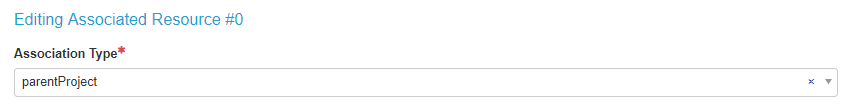
\includegraphics{images/product_association_type.png}

\textbf{Step 2}: Click the \textbf{Select a Record} button to select an associated project.

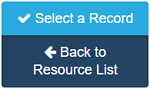
\includegraphics{images/select_a_record_button.png}

\textbf{Step 3}: Choose the project that you would like to associate from the \textbf{Select a Resource} list.

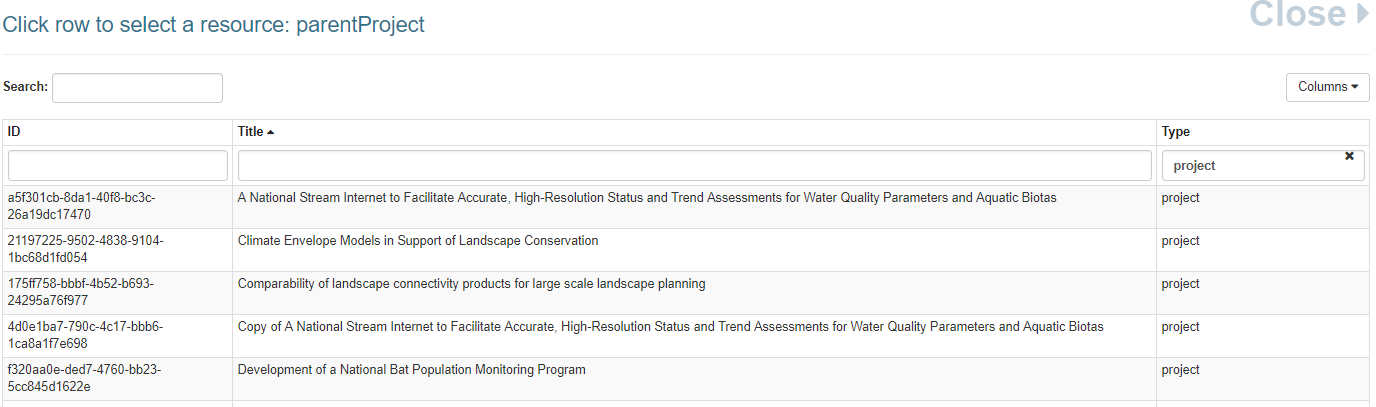
\includegraphics{images/product_association_choose_parent.png}

\textbf{Step 4}: Fill out the Linked Association Type with \textbf{product}.

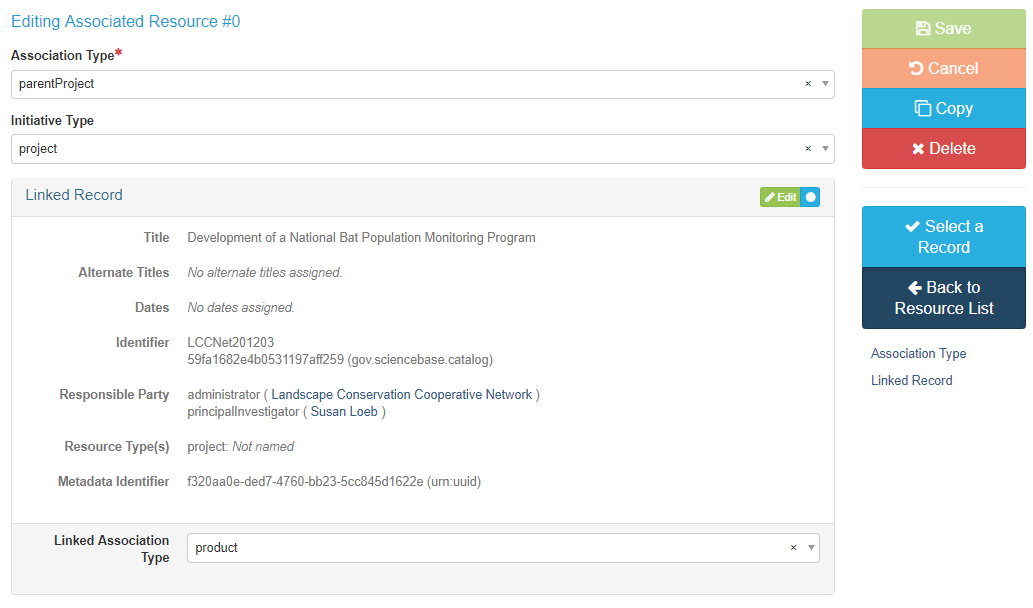
\includegraphics{images/product_association_linked_record.png}

\hypertarget{help}{%
\chapter{Help}\label{help}}

{[}Under development{]}

\hypertarget{glossary}{%
\chapter{Glossary of Terms}\label{glossary}}

\hypertarget{adiwg}{%
\section{ADIwg}\label{adiwg}}

Alaska Data Integration working group

\hypertarget{auto-save}{%
\section{Auto-Save}\label{auto-save}}

A feature in mdEditor settings that allows information to be automatically saved as it is entered. Consult the \protect\hyperlink{settings}{Settings} section of this manual for more information.

\hypertarget{customization}{%
\section{Customization}\label{customization}}

The ability afforded by open-source code to edit the code of an application (in this case mdEditor) according to the needs of the users.

\hypertarget{fgdc}{%
\section{FGDC}\label{fgdc}}

Federal Geographic Data Committee \url{https://www.fgdc.gov/}

\hypertarget{fgdc-csdgm}{%
\section{FGDC CSDGM}\label{fgdc-csdgm}}

Federal Geographic Data Committee's Content Standard for Digital Geospatial Metadata - FGDC-STD-001-1998 Includes Biological Data Profile \url{https://www.fgdc.gov/metadata/csdgm/}

\hypertarget{html}{%
\section{HTML}\label{html}}

HTML stands for Hyper Text Markup Language. It is the standard markup language for creating Web pages. HTML is the `human-readable' and printable report of the metadata content

\hypertarget{iso}{%
\section{ISO}\label{iso}}

International Organization for Standardization - ISO is an independent, non-governmental international organization with a membership of 162 national standards bodies.

Through its members, it brings together experts to share knowledge and develop voluntary, consensus-based, market relevant International Standards that support innovation and provide solutions to global challenges.

\hypertarget{iso-19110}{%
\subsection{ISO 19110}\label{iso-19110}}

International Standards Organization Geographic Information - Feature Catalogue 19110:2005

ISO 19110 defines the methodology for cataloguing feature types. It may be used as a basis for defining the universe of discourse being modelled in a particular application, or to standardize general aspects of real world features being modelled in more than one application. (International Organization for Standardization (2016). ISO 19110:2016. Retrieved from: \url{https://www.iso.org/standard/57303.html})

\hypertarget{iso-19115-1}{%
\subsection{ISO 19115-1}\label{iso-19115-1}}

Defines the schema required for describing geographic information and services by means of metadata. It provides information about the identification, the extent, the quality, the spatial and temporal aspects, the content, the spatial reference, the portrayal, distribution, and other properties of digital geographic data and services. (International Organization for Standardization (2014). ISO 19115-1:2014. Retrieved from: \url{https://www.iso.org/standard/53798.html})

\hypertarget{iso-19115-2}{%
\subsection{ISO 19115-2}\label{iso-19115-2}}

International Standards Organization Geographic Information - Metadata 19115-2:2009
Extends the existing geographic metadata standard by defining the schema required for describing imagery and gridded data. It provides information about the properties of the measuring equipment used to acquire the data, the geometry of the measuring process employed by the equipment, and the production process used to digitize the raw data. This extension deals with metadata needed to describe the derivation of geographic information from raw data, including the properties of the measuring system, and the numerical methods and computational procedures used in the derivation. The metadata required to address coverage data in general is addressed sufficiently in the general part of ISO 19115. (International Organization for Standardization (2009). ISO 19115-2:2009. Retrieved from: \url{https://www.iso.org/standard/39229.html})

\hypertarget{json}{%
\section{JSON}\label{json}}

Javascript Object Notation, a general purpose format like CSV.

\hypertarget{keywords}{%
\section{Keywords}\label{keywords}}

Words used in an information retrieval system to indicate the content of a document.

\hypertarget{localstorage-cache}{%
\section{localStorage Cache}\label{localstorage-cache}}

localStorage Cache allows an application to store data locally, in a user's browser. Storing information on the browser's local storage cache (instead of a normal file cache) means that if you use a different browser to access the mdEditor, it will not show the data you've imported from your first browser. It also means that if you clear your browser's cache, it will generally not clear your mdEditor records. However, depending upon your browser settings (E.g., in Chrome, if the ``cookies and other site data'' option is checked), clearing your browser cache may still clear your mdEditor data.

\hypertarget{mdeditor}{%
\section{mdEditor}\label{mdeditor}}

Web application for authoring and editing metadata, for both projects and products.

\hypertarget{mdeditor-file}{%
\section{mdEditor File}\label{mdeditor-file}}

A mdJSON file created by mdEditor that contains all of the information contained in mdJSON, along with mdEditor settings. This can be exported and shared with collaborators, imported into another record set, or saved to a local workstation as a backup or archival copy.

\hypertarget{mdjson}{%
\section{mdJSON}\label{mdjson}}

ADIwg standard for encoding project and data metadata, based on JavaScript Object Notation (JSON).

\hypertarget{mdjson-file}{%
\section{mdJSON File}\label{mdjson-file}}

An mdJSON file that is proprietary to the Metadata toolkit developed by the Alaska Data Integration Working Group (ADIWG), learn more at {[}\url{https://adiwg.github.io/mdTools/}{]}.

\hypertarget{mdtranslator}{%
\section{mdTranslator}\label{mdtranslator}}

Open-source Ruby software application for translating between metadata standards. Metadata is input in one of the supported `reader' formats and output in one of the supported `writer' formats. Available as Ruby gem or Command-Line-Interface.

Metadata is a set of data that describes and gives information about other data.

A server where metadata is published to.

\hypertarget{parentid}{%
\section{ParentID}\label{parentid}}

Identifier for a folder on a database where records will be stored upon publishing.

\hypertarget{sbjson}{%
\section{sbJSON}\label{sbjson}}

U.S. Geological Survey's standard for documenting records ingested into ScienceBase Catalog. The format used to define the attributes of ScienceBase items.

\hypertarget{sciencebase}{%
\section{ScienceBase}\label{sciencebase}}

A USGS collaborative scientific data and information management platform used directly by science teams. ScienceBase provides access to aggregated information derived from many data and information domains, including feeds from existing data systems, metadata catalogs, and scientists contributing new and original content. ScienceBase architecture is designed to help science teams and data practitioners centralize their data and information resources to create a foundation needed for their work. ScienceBase, both original software and engineered components, is released as an open source project to promote involvement from the larger scientific programming community both inside and outside the USGS. (USGS (2018). About ScienceBase. Retrived from: \url{https://www.sciencebase.gov/about/content/about-sciencebase}).

\hypertarget{uri}{%
\section{URI}\label{uri}}

Uniform Resource Identifier is a string of characters used to identify a resource. A URL is a type of URI.

  \bibliography{book.bib,packages.bib}

\printindex
\backmatter

\end{document}
